\documentclass[10pt, a4paper,twoside]{scrartcl}
\usepackage[ngerman]{babel}
\usepackage{amsmath}
\usepackage{amssymb}
\usepackage{graphicx}
\usepackage{subcaption}
\usepackage{float}
\usepackage[top=2cm,bottom=3cm,outer=2cm,inner=3cm]{geometry}\usepackage[utf8]{inputenc}
\usepackage{hyperref}
\usepackage[multiple]{footmisc}
\usepackage{parskip}
\usepackage{wrapfig}
\usepackage{xfrac}
\usepackage{xcolor}
\usepackage{tikz}
\usetikzlibrary{arrows}
\usetikzlibrary{arrows.meta}
\usepackage{longtable}
\usepackage{pdfpages}
\usepackage[tikz]{bclogo}
\usepackage{eurosym}

\hypersetup{
    colorlinks=true,
    linkcolor=blue,
    filecolor=magenta,      
    urlcolor=cyan
}

\restylefloat{table}

\newcommand{\warn}[1]{\textbf{#1}}
\newcommand{\con}[1]{\texttt{#1}}
\newcommand{\dis}[1]{\textbf{\texttt{#1}}}

\newenvironment{remember}{\begin{bclogo}[couleur=blue!30,arrondi=.1,logo=\bccrayon,ombre=true]{Merke}}{\end{bclogo}}   
\newenvironment{remark}{\begin{bclogo}[couleur=blue!30,arrondi=.1,logo=\bcinfo,ombre=true]{Hinweis}}{\end{bclogo}}   
\newenvironment{warning}{\begin{bclogo}[couleur=red!30,arrondi=.1,logo=\bcattention,ombre=true]{Warnung}}{\end{bclogo}}   


\title{QRP CW Transceiver Baumappe}
\subtitle{Board Rev. 2, Firmware Rev. 2.0}
\author{Hannes Matuschek -- DM3MAT\\\texttt{<dm3mat [at] darc [dot] de>}\\\texttt{https://dm3mat.darc.de/cw2019}}
\date{\today}

\begin{document}
\maketitle

\begin{abstract}
Diese Baumappe beschreibt den Zusammenbau, Abgleich und die Bedienung der zweiten Revision meines kleinen, portablen CW TRX. Wenn Sie keinen \emph{rev 2} Aufdruck auf den Leiterplatten finden können, ist dies das falsche Dokument!

Der Hauptunterschied zwischen dieser und der ersten Revision ist der Mischer. Anstatt des \texttt{74HC4053}, der eine recht große Dämpfung bei höheren Frequenzen aufweist, verwendet die zweite Revision den \texttt{FST3253}. Dieser Mischer kann problemlos bis ins 10m Band verwendet werden. Außerdem wurde das Platinenlayout vereinfacht. Die Platinen werden nun durch Platinensteckverbinder verbunden, was den Aufbau des TRX deutlich vereinfacht. Auch wanderte der Mikrocontroller auf die Empfängerplatine. Es gibt nun nur noch zwei Platinen mit $10\times 8\,cm$ Abmaßen und nicht mehr drei. Diese passen gerade so in ein Fischer-Gehäuse (\texttt{KOH-2100} + \texttt{KOH-4100} + \texttt{DPL 2-4}).
\end{abstract}
\thispagestyle{empty}
\vfill
\begin{center}
 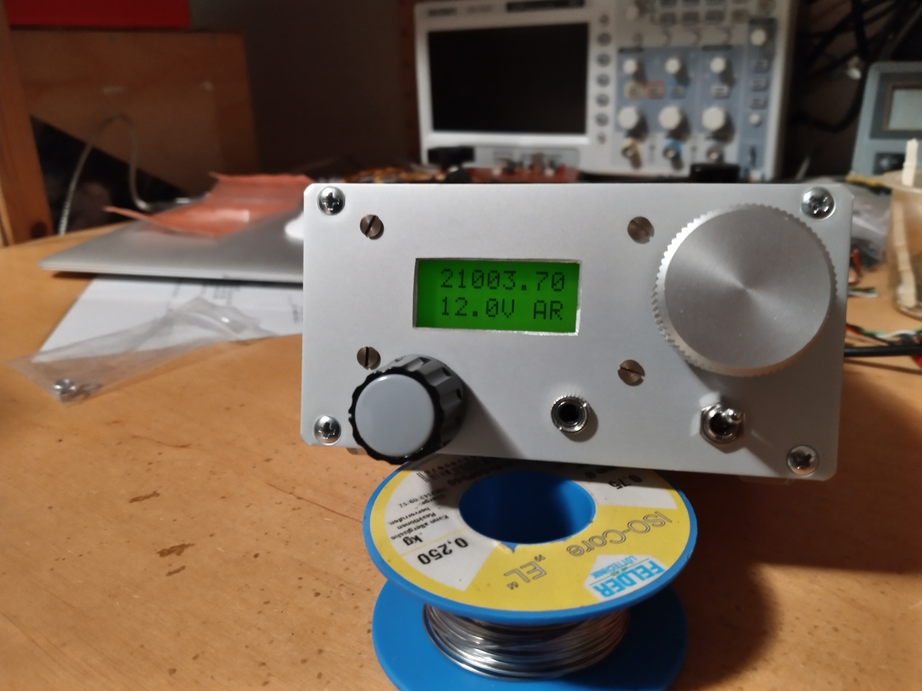
\includegraphics[width=0.7\linewidth]{fig/complete_small.png}
\end{center}



\cleardoublepage
\tableofcontents
\thispagestyle{empty}

\cleardoublepage
\section{Empfänger- \& Controllerplatine} \label{sec:rx}
 Auf dieser Platine befindet sich der Hauptteil der gesamten TRX-Schaltung. Der Empfänger ist ein Direktüberlagerungsempfänger (Driektmischer), der einen \texttt{FST3253} CMOS-Schalter als so genannter \emph{sample-hold} Mischer verwendet (zusammen mit \texttt{C4-C7}). Dieser Mischer benötigt zwei VFO Signale mit $90^\circ$ Phasendifferenz und produziert vier Mischprodukte mit $0^\circ$, $90^\circ$, $180^\circ$ und $270^\circ$ Phasenverschiebung. Diese zwei Signalpaare ($0^\circ$ + $180^\circ$) und ($90^\circ$ + $270^\circ$) werden dann in zwei unabhängige Differenzverstärker (\texttt{U6A}, \texttt{U6B}) geführt, die zwei um $90^\circ$ phasenverschobene Audiosignale produzieren (für USB, $-90^\circ$ für LSB). Das nachfolgende Phasennetzwert \texttt{U7} \& \texttt{U8} verschiebt dann die Phasenlage der Audiosignale um $-90^\circ$ bei $700\,Hz$. Zuletzt werden die resultierenden Signale mit \texttt{RV3} addiert. Dabei interferieren USB-Signale konstruktiv und LSB-Signal heben sich auf. Diese \emph{Phasenmethode} erlaubt Direktüberlagerungsempfängern eine Unterdrückung eines Seitenbanden. Die weiteren Audiostufen (\texttt{U3} \& \texttt{U5}) filtern und verstärken Audiosignale nahe $700\,Hz$, welche schließlich in die Audio-PA \texttt{U4} geführt werden.
 
 Der Controller- und VFO-Abschnitt der Platine besteht aus einem \texttt{ATMega 328P} Mikrocontroller, der die \texttt{SI5351} PLL steuert. Das \texttt{CLK2} Signal der PLL treibt zwei Flip-Flops \texttt{U9}, welche die Frequenz des \texttt{CLK2} Signals durch vier teilen und dabei zwei um $90^\circ$ phasenverschobene VFO-Signale für den Mischer erzeugen.
  
\subsection{Aufbau des Controllers}
 In einem ersten Schritt wird der Controllerteil der Platine aufgebaut. Löten Sie \texttt{C2}, \texttt{C26}, \texttt{J7} Steckverbinder, \texttt{L2}, \texttt{C40}, \texttt{C41}, \texttt{C42}, \texttt{U10}, \texttt{J10}, \texttt{C14}, \texttt{J3}, \texttt{R3}, \texttt{C46}, \texttt{R4}, \texttt{U11} + Socket, \texttt{LCD1} Steckverbinder, \texttt{R43}, \texttt{R5}, \texttt{RV4}, \texttt{J9} Steckverbinder, \texttt{R41}, \texttt{R40}, \texttt{C39} \& \texttt{U9} ein. 

\begin{remark}
 Durch das kompakte Design sind die Bauteilreferenzen leider teilweise schlecht zu lesen. I habe dafür, mit Hilfe eines sehr netten KiCAD Plugins, eine \href{https://dm3mat.darc.de/cw2019/rx_rev2_ibom.html}{interaktive BOM} für diese Platine exportiert. Damit sollte es recht einfach sein, bestimmte Bauteile auf der Platine zu finden.
\end{remark}

\begin{warning}
Das Metallfähnchen des TO-220 Gehäuses von \texttt{U10} ist üblicherweise direkt mit dem Mittelpin (GND) verbunden. Bitte prüfen Sie das vor dem Einbau. Einige sehr seltene Varianten verbinden dieses Fähnchen mit $+5\,V$, was einen soliden Kurzschluss verursacht.
\end{warning}

Wenn Sie einen der seltenen Varianten von \emph{U10} verwenden, fügen Sie bitte ein Glimmerplätchen zwischen dem TO-220 und der Leiterplatte ein um einen Kurzschluss zu verhindern. Falls nicht, kann darauf verzichtet werden und U10 direkt auf die Platine verschraubt werden.

 \texttt{R43} limitiert den Strom zur LCD-Hintergrundbeleuchtung. Standardmäßig wird hier ein $220\,\Omega$ Widerstand verwendet. Dieser limitiert den Strom auf ungefähr $23\,mA$. Die führt zu eine sehr schwachen Hintergrundbeleuchtung verringert aber den Stromverbrauch von den max. $120\,mA$ (\texttt{R43} kurzgeschlossen). Ich finde persönlich eine schwache Hintergrundbeleuchtung ideal: Während der Nacht reicht auch eine geringe Hintergrundbeleuchtung aus um das Display lesen zu können. Am Tage ist diese Beleuchtung völlig unnötig. Eine sehr helle Hintergrundbeleuchtung ist daher nicht notwendig und würde nur unnötig viel Batteriestrom verbrauchen. Wenn Sie diesen TRX ausschließlich zu Hause verwenden, können Sie \texttt{R43} überbrücken um somit die maximale Helligkeit zu erhalten.
 
\begin{remark} 
 Sie können auch den Widerstand \texttt{R43} mit einem Taster am Frontpanel ersetzen um die Hintergrundbeleuchtung bei bedarf einzuschalten.
\end{remark}

 Als nächsten bauen Sie den Stecker für den Schalter zusammen (oben-rechts auf der Platine mit der Beschriftung \texttt{SW}). Verbinden Sie eine $12\,V$ Spannungsquelle (Strombegrenzt auf nicht mehr als $100\,mA$) mit den Pads oben-rechts auf der Leiterplatte mit der Beschriftung \texttt{+ G}, wobei \texttt{+} $+12\,V$ und \texttt{G} Masse bedeutet.

\begin{remember}
 Die Empfängerplatine selbst besitzt keine Absicherung gegen Verpolung. Seien Sie also vorsichtig, wenn Sie den RX an die Spannungsquelle anschließen.
\end{remember}

 Wenn nichts in Rauch aufgeht, schalten Sie den RX aus und bauen sie die Stecker für den Drehimpulsgeber und das LCD auf.  

 Der Stecker für den Drehimpulsgeber hat die folgenden Anschlüsse (von links nach rechts) \emph{Mitteltaster}, \emph{Encoder B}, \emph{Encoder A} und \emph{Masse}.

 Der LCD-Stecker hat die folgenden Anschlüsse (von links nach rechts): \emph{5V} Pin 2 am LCD, \emph{Kontrast} Pin 3 am LCD, \emph{LED Hintergrundbeleuchtung} Pin 15 am LCD, \emph{GND} Pin 1 am LCD, \emph{RS (register selection)} Pin 4 am LCD, \emph{D4-D7} Pins 11-14 am LCD, \emph{Chip-Enable (EN)} Pin 6 am LCD. Sie müssen auch Pins 5 und 16 direkt am LCD mit Masse (Pin 1, GND) verbinden.
 
 Verbinden Sie nun den Drehimpulsgeber und das LCD mit der Platine und installieren Sie den \texttt{ATMega328} Mikrocontroller. Dann verbinden Sie den RX wieder mit der Spannungsversorgung. Wenn Sie einen vorprogrammierten MCU erhalten haben, sollten Sie nun eine kurze Begrüßung auf dem Display lesen können. Wenn Sie gar nichts oder eine Reihe schwarzer Blöcke auf dem Display sehen, sollten sie zunächst den Kontrast mit \texttt{RV4} einstellen. Wenn Sie weiterhin nichts auf dem Display sehen, überprüfen Sie bitte die Verbindungen zwischen der Platine und dem Display.

\subsection{Die PLL Testen}
 Als nächstes wird die Funktion der \texttt{SI5351} PLL überprüft. Dazu stecken Sie das \texttt{SI5351} breakout-board in den Sockel J9.

\begin{warning}
 Bitte achten Sie darauf, das \texttt{SI5351} beakout-board richtig herum einzusetzen. Es gibt keinen Schutz. Das breakout-board sollte mit dem LCD Steckverbinder überlappen nicht aber \texttt{U9}!
\end{warning}
 
 Schalten Sie nun den RX ein und überprüfen Sie ob ei $3.5\,MHz$ Signal an den Pins 8, 9, 11 und 12 von \texttt{U9} anliegt. Wenn nicht, überprüfen Sie ob ein $14.0\,MHz$ Signal am \texttt{CLK2} Ausgang des \texttt{SI5351} beakout-board anliegt. An dieser Stelle können Sie auch die $90^\circ$ Phasenverschiebung zwischen den Pins 8 und 12 von \texttt{U9} überprüfen.

\begin{remark}
Standardmäßig ist der RX für den Empfang des oben Seitenbandes (USB) ausgelegt. Wenn Sie den LSB Empfang bevorzugen, unterbrechen Sie die Verbindung des Jumpers \texttt{USB} und überbrücken Sie den Jumper \texttt{LSB} neben \texttt{U9}.
\end{remark} 

Wenn alles zu Ihrer Zufriedenheit funktioniert, fahren Sie mit dem Zusammenbau des restlichen Empfängers fort.


\subsection{Aufbau des Empfängers}
Bevor Sie mit dem Zusammenbau des Empfängers fortfahren, entfernen Sie alle Verbindungen zur Platine. Das heißt, entfernen Sie den \texttt{SI5351}, das LCD und den Impulsgeber sowie die Verkabelung zur Spannungsversorgung.

Als erstes sollte der SMD SOIC-16 \texttt{FST3253} Mischer eingelötet werden. 

\begin{warning}
 Seien Sie vorsichtig! Der \texttt{SI5351} sowie der \texttt{FST3253} sind \textbf{sehr} empfindlich gegenüber elektrostatischer Entladung. Tragen Sie ein anti-static Armband und verwenden Sie eine anti-statische Matte. Tragen Sie keine Kleidung aus Wolle oder synthetischen Fasern. Ich habe schon zwei \texttt{FST3253} auf diese Weise zerstört. 
\end{warning}

\paragraph{Falls Sie noch nie SMD Komponenten verbaut haben}
 Es ist überraschend einfach. Verwenden Sie eine kleine Spitze für Ihren Lötkolben, dünnes Lötzinn (z.B., $0.75mm$) und reichlich Flussmittel! Geben Sie eine gute Portion Flussmittel auf die Pads und Verzinnen Sie ein Pad (z.B., Pin 1). Dann nehmen Sie den IC mit einer spitzen Pinzette auf und fixieren Sie ihn ausschließlich an Pin 1 indem Sie das Pad erhitzen und den IC auf die Platine drücken. Überprüfen Sie nun die Ausrichtung des IC mit seinen Pads. Ist alles zu ihrer Zufriedenheit, können Sie die verbleibenden Pins verlöten. Verwenden Sie wenig Lötzinn und lassen Sie das Flussmittel die ganze Arbeit machen! Falls Sie eine Lötbrücke zwischen zwei Pins erhalten, entfernen Sie das überschüssige Lötzinn mit etwas Entlötlitze.

Sobald der Mischer installiert ist, ist die Reihenfolge, in der die  weiteren Bauelemente installiert werden unkritisch. Bauen Sie den restlichen RX auf, lassen Sie aber noch die Platinensteckverbinder sowie die RCA-Buchse (\texttt{TX-OC}) weg. Diese werden erst am Ende montiert.

\begin{remark}
Die Audio-PA (\texttt{LM386}, \texttt{U4}) hat sehr viel Verstärkung. Wenn Sie lediglich Kopfhörer verwenden wollen, können Sie \texttt{R13} und \texttt{C16} weglassen. Sie könne sie später noch hinzufügen.
\end{remark}

Um den Eingangstransformator zu wickeln, schneiden sie drei 15-16 cm lange CuL-Drahtstücke zurecht. Starten Sie die Windungen indem Sie die drei Drähte \textbf{von Hinten} durch den Kern stecken. Halten Sie diese nun fest und machen Sie die nächste Windung indem Sie die Drähte gegen den Uhrzeigersinn \textbf{von vorn} durch den Kern stecken. Fahren Sie nun fort bis sie 8 Findungen gegen den Uhrzeigersinn auf den Kern gebracht haben. Jedes mal, wenn die Drähte durch den Kern gesteckt werden, gilt als eine Windung.

\begin{figure}[ht!]
 \begin{subfigure}[t]{0.49\textwidth}
   \centering
   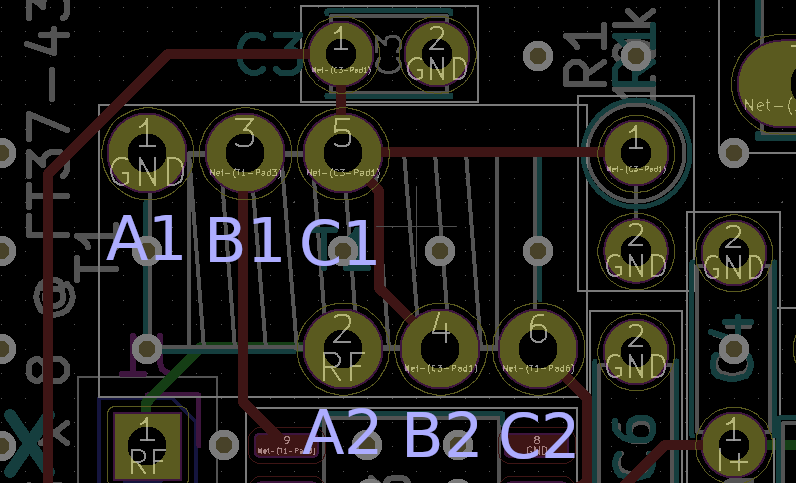
\includegraphics[width=0.9\textwidth]{fig/RX_T1.png}
   \caption{Footprint von T1}
 \end{subfigure}
 \begin{subfigure}[t]{0.49\textwidth}
   \centering
   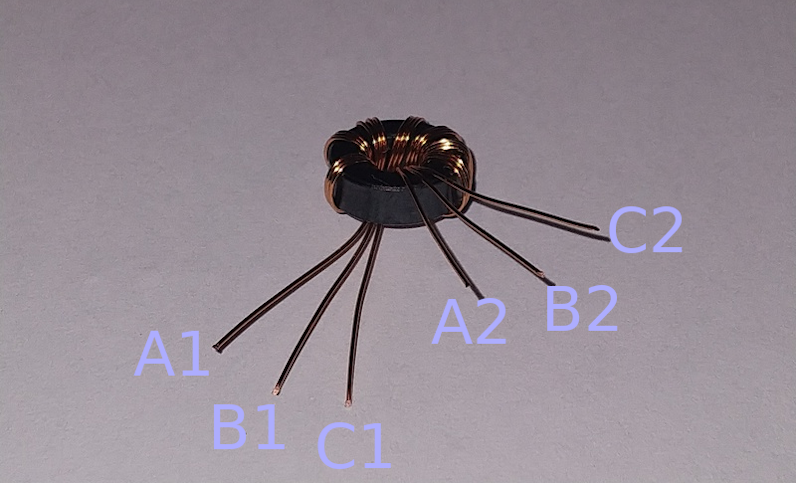
\includegraphics[width=0.9\textwidth]{fig/RX_T1_IMG_small.png}
   \caption{Gewickelter T1 mit Beschriftung.}
 \end{subfigure}
 \caption{Bevor Sie den Transformator einlöten, überprüfen Sie bitte korrekte Ausrichtung der Anschlüsse. Das Bedeutet das oben-linke wird mit dem unten-linken (d.h., A1 mit A2), oben-mitte mit dem unten-mitte (d.h., B1 mit B2) und das oben-rechte mit dem unten-rechten Pad (d.h., C1 mit C2) verbunden ist.}
\end{figure}

\begin{warning}
Die Audioendstufe neigt leider zum Schwingen, vor allem wenn ein kleiner Lautsprecher verwendet wird. Wenn das passiert, wird der gesamte Audiopfad in die Sättigung getrieben. Dabei kann bis zu 12V an den Mixer geführt werden, was diesen dann zerstört! Um das zu verhindern, \textbf{sollten} vier 5.1V Zenerdioden parallel zu den Kondensatoren C4-C7 fliegend gelötet werden. 
\end{warning}

\subsection{Empfängertest und Abstimmung}
Sobald der Empfänger vollständig aufgebaut ist, verbinden Sie die Spannungsversorgung und bereiten Sie die Stecker für die Lautstärke und den Kopfhörerausgang vor. Verbinden Sie nun auch ein Stück Koaxialkabel mit den \texttt{RX}/\texttt{GN} Pads links-oben auf der Platine. Dies ist der Antenneneingang für den Test. Je nachdem welches Band Sie gewählt haben, sollten Sie die Strombegrenzung der Spannungsversorgung nun auf $120\,mA$ erhöhen.

\subsubsection{Frequenzabstimmung}
Wenn ein genauer Frequenzzähler vorhanden ist, können Sie mit der Feinabstimmung der PLL Frequenz anfangen. Wählen Sie dazu im Menu das 20m Band aus und stellen Sie eine Frequenz von $14.000.70 MHz$ ein. Messen Sie nun die Frequenz am USB Pad. Sie Sollte nun genau $14.0\,MHz$ betragen (falls die Seitentonfrequenz auf $700\,Hz$) eingestellt ist. Sollte die Frequenz abweichen, wählen Sie im \emph{Setup}-Menü den Punkt \emph{PLL correction}. Sie können nun die PLL-Korrektur einstellen bis Sie die gewünschte Frequenz messen.

\subsubsection{CW Filter Abgleich}
Ach wenn die Mittenfrequenz des CW Audiofilter von $\approx 700\,Hz$ nicht geändert werden kann, werden Variationen in den Bauelementwerten zu eine kleinen Verschiebung der Mittenfrequenz des schmalen Filters führen. Für einen guten Abgleich der Send- und Empfangsfrequenzen sollte der CW Seitenton auf genau der Mittenfrequenz des CW Filters liegen. Daher sollte das Spektrum des CW Filters gemessen werden. Zum Beispiel mit der PC Soundkarte und einer Anwendung, die dieses Spektrum darstellt. Die so ermittelte Mittenfrequenz des CW Filters sollte dann unter \texttt{Menu}\ $\rightarrow$\ \texttt{Setup}\ $\rightarrow$\ \texttt{CW Tone} eingestellt werden.

\begin{remember}
Die im Display dargestellte Frequenz ist die Frequenz auf dem der TRX sendet. Nicht die VFO-Frequenz während des Empfangs.
\end{remember}

\subsubsection{Seitenbandunterdrückung}
Wenn Sie über einen Signalgenerator verfügen, stellen Sie ihn auf $14.000 MHz$ ein. Verbinden Sie den Signalgenerator über ein geeignetes Dämpfungsglied mit dem RX. Wählen Sie dann das 20m Band aus und stimmen Sie auf $14.001.3\,MHz$ ab. Sie werden nun einen sehr niedrigen Ton (c.a. $500\,Hz$) hören. Stimmen Sie nun \texttt{RV2} \& \texttt{RV3} ab um die Lautstärke dieses Tons zu minimieren. Dann stimmen Sie den RX auf $14.001.6\,HMz$ ab. Sie sollte nun eine hohen Ton ($900\,Hz$) hören. Stimmen Sie nun \texttt{RV1} \& \texttt{RV3} ab um die Lautstärke dieses Tons zu minimieren. Es könnte notwendig sein, diese Vorgang abwechselnd zu wiederholen bis ein optimales Ergebnis erreicht wird.

Mit diesem Abgleich ist der Abgleich des RX nun vollständig. 

\clearpage
\subsection{RX Bauelemente}  \label{sec:rxcomp}
\begin{longtable}{|l|p{6cm}|l|l|} \hline 
\# & Component & Value & Remarks \\ \hline 
1 & R15 & 10R & \\
4 & R20, R21, R22, R23 & 100R & \\
1 & R43 & 220R & \\
3 & R38, R39, R42 & 1k & \\
1 & R13 & 2.2k & \\
9 & R7, R27, R29-R31, R33, R35-R37 & 3.3k & \\
1 & R32 & 4.3k & \\
1 & R4 & 4.7k & \\
1 & R26 & 5.1k & \\
1 & R34 & 7.5k & \\
10 & R1, R2, R6, R11, R18, R24, R25, R28, R40, R41 & 10k & \\
2 & R9, R10 & 30k & \\
2 & R12, R14 & 33k & \\
2 & R16, R17 & 36k & \\
2 & R3, R5 & 47k & \\
1 & R8 & 120k & \\
1 & R19 & 470k & \\
2 & RV1, RV2 & 50k & \\
1 & RV3 & 500R & \\
1 & RV4 & 10k & \\
3 & C13, C20, C23 & 1n & \\
2 & C25, C27 & 3.3n & \\
3 & C30, C31, C35 & 10n & \\
5 & C12, C17, C18, C21, C33 & 47n & \\
23 & C3, C8, C11, C22, C24, C26, C29, C32, C34, C37-C41, C46-C54 & 100n & \\
5 & C4, C5, C6, C7, C36 & 470n & \\
2 & C1, C28 & 1u & \\
3 & C15, C16, C42 & 10u & \\
3 & C2, C14, C19 & 100u & \\
6 & L1, L3, L4, L5, L6, L7, L8, L9 & 100u & \\
1 & T1 & 3 x 8 @ FT37-43 & \\
1 & D1 & 1N4148 & \\
4 & parallel zu C4-C7 & 5.1V Zener & \\
1 & Q1 & BS170 & \\
1 & Q2 & 2N3904 & \\
1 & U1 & FST3253 & \\
5 & U3, U5, U6, U7, U8 & LM833 & \\
1 & U4 & LM386 & \\ 
6 & -- & DIP-8 Sockets & \\
1 & U9 & 74AC74 & \\
1 & U10 & L7805 & \\
1 & U11 & ATmega328-PU & \\
1 & --  & DIP-28 Socket & \\
1 & - & SI5351 break-out & \\
2 & J1, J3, J4, J11 & 1x10 pin-header long & \\
1 & J6 & 2x3 pin-header & \\
1 & J9 & 1x7 pin-socket & \\
2 & J2, J7 & 1x2 90deg & \\
1 & -- & Switch & \\
1 & J8 & 1x3 90deg & \\
1 & -- & 10k log & potentiometer \\
1 & J10 & 1x4 90deg & \\
1 & -- & Rotary encoder & \\
1 & LCD1 & 1x10 90deg & \\
1 & -- & LCD & 2 x 8 symbols \\
1 & J13 & TX-OC & RCA-jack (optional) \\
1 & J5 & Key & 3.5mm stereo jack\\ \hline
\end{longtable}


\cleardoublepage
\section{PA \& Tiefpassfilter-Platine} \label{sec:pa}
Den Hauptteil der PA/LP-Platine wird von den vier 7-Pol Chebyschev Tiefpassfilter eingenommen. Diese Chebyschevfilter werden benötigt um mit lediglich vier Tiefpassfiltern alle HF-Bänder von 80m bis 10m abzudecken. Der Filter ganz rechts deckt die 80m und 60m Bänder ab und sollte eine Grenzfrequenz von $5.6\,MHz$ haben. Der nächste Filter deckt das 40m und 30m Band ab und sollte eine Grenzfrequenz von $10.5\,MHz$. Der vorletzte Filter deckt das 20m und 17m Band ab und sollte eine Grenzfrequenz von $20\,MHz$ haben. Letztendlich der Filter ganz links deckt das 15m, 12m und 10m Band ab und sollte eine Grenzfrequenz von $30\,Mhz$. Die einzelnen Tiefpassfilter werden mit 4 Subminiaturrelais umgeschaltet die von der RX Platine durch \texttt{J2} gesteuert werden.

Der MOSFET \texttt{Q4} fungiert als RX/TX-Schalter, der das Tiefpass-gefilterte Signal vom Eingang zum RX über \texttt{J6} führt. Der PA-Abschnitt besteht aus einem \texttt{74HCT00} als Treiber und vier \texttt{BS170} MOSFETs als PA Transistoren. Das TX-Oszillator-Signal kommt von der RX/Controller-Platine via \texttt{J7}. Die Stromversorgung des gesamten TRX geschieht durch die Buchse \texttt{J3} und die Stromversorgung des RX erfolgt durch \texttt{J11}.

\begin{remark}
 Bevor Sie die Tiefpassfilter auf die Platine löten, bauen Sie diese zuerst auf einem Stück Leiterplattenmaterial auf und messen Sie diesen durch. Chebyschev Tiefpassfilter sind etwas empfindlich bezüglich der Komponentenwerte.
\end{remark}

 Wenn keine Messgeräte vorhanden sind, ziehen Sie bitte jeweils eine Windung von den gegebenen Werten ab. Die Anzahl der Windungen wurden aus den Al-Werten des Herstellers bestimmte. Meiner Erfahrung nach führt dies zu leicht zu großen Induktivitäten. Außerdem gehen Sie sicher lieber das Risiko einer zu hohen als einer zu niedrigen Grenzfrequenz der Tiefpassfilter ein. 
 
\begin{remark}
 Wie für die Empfängerplatine, gibt es auch für die PA-Platine eine \href{https://dm3mat.darc.de/cw2019/pa_rev2_ibom.html}{interaktive BOM}.
\end{remark}

 Die Diode \texttt{D4} ist parallel in Sperrrichtung zur Spannungsversorgungsbuchse geschaltet. Zusammen mit einer Sicherung im Kabel dient diese Diode dem Verpolschutz. Wenn die Spannungsversorgung falsch herum angeschlossen wird, schließt diese Diode die Spannungsversorgung kurz, was die Sicherung in der Versorgungsleitung durchbrennen lässt. Eine 2A Sicherung \emph{flink} sollte es schon sein. 

 Zuletzt löten Sie die Platinensteckverbindersockel \texttt{J2}, \texttt{J6}, \texttt{J7} ein \texttt{J11}.
´ 
\clearpage
\subsection{PA/Tiefpass Bauelemente}  \label{sec:pacomp}
\begin{longtable}{|l|p{6cm}|l|l|} \hline 
\# & Component & Value & Remarks \\ \hline 
2 & R12, R13 & 100 & \\
1 & R9 & 470R & \\
1 & R10 & 1k & \\
1 & R14 & 4.7k & \\
7 & R1, R3, R5, R7, R11, R15, R16 & 10k & \\
4 & R2, R4, R6, R8 & 100k & \\
2 & C2, C15 & 100p & NP0 \\
4 & C3, C6, C11, C16 & 220p & NP0 \\
4 & C4, C7, C12, C17 & 470p & NP0 \\
2 & C5, C18 & 820p & NP0 \\
2 & C8, C13 & 1n & NP0 \\
2 & C9, C14 & 1.5n & NP0 \\
11 & C1, C10, C19, C20, C22, C23, C24, C27, C28, C29, C30 & 100n & \\
1 & C25 & 1u & \\
1 & C26 & 220u & \\
1 & L14 & 22u & 07HCP \\
1 & L13 & 100u & MICC \\
3 & L1, L5, L9 & 330n & 11T on T37-6 \\
3 & L2, L6, L10 & 480n & 13T on T37-6 \\
3 & L3, L7, L11 & 750n & 14T on T37-2 \\
3 & L4, L8, L12 & 1700n & 21T on T37-2 \\
1 & T1 & -- & 8T + 8T on FT37-43 \\
4 & K1, K2, K3, K4 & G6S-2 & \\
6 & D1, D2, D3, D5, D6, D7 & 1N4148 & \\
1 & D4 & 1N4001 & \\	
4 & Q1, Q2, Q3, Q10 & 2N3904 & \\
6 & Q4, Q6, Q7, Q8, Q9, Q11 & BS170 & \\
1 & Q5 & BD140-16 & \\
1 & U1 & 74HCT00 & \\
1 & J1 & BNC & \\
1 & J2 & 1 x 8 pin-socket & \\
1 & J3 & barrel-jack & \\
3 & J6, J7, J11 & 1 x 2 pin-socket & \\ \hline
\end{longtable}


\cleardoublepage
\section{Endmontage} \label{sec:box}
Schließlich folgt die Endmontage. In diesem schritt werden die Platinensteckverbinder montiert. Wie dies geschieht hängt ein wenig von dem Verwendeten Gehäuse ab. Die Beschreibung die ich hier gebe, betrifft den Fischer-Gehäusebausatz \texttt{KOH-2100} + \texttt{KOH-4100} + \texttt{DPL 2-4}. Dieses ist ein kompaktes $10 \times 10 \times 5\,cm$ Gehäuse. Die Platinen werden mit c.a. $\approx 1.5\,cm$ Abstand in die untere Halbschale geschoben. Leider habe ich keine passenden Stapelleisten für diesen Abstand gefunden und verwende daher welche mit $38\,mm$ Gesamtlänge und daher die viel zu lang sind.

\begin{figure}[!ht]
 \centering
 \begin{subfigure}{0.49\linewidth}
  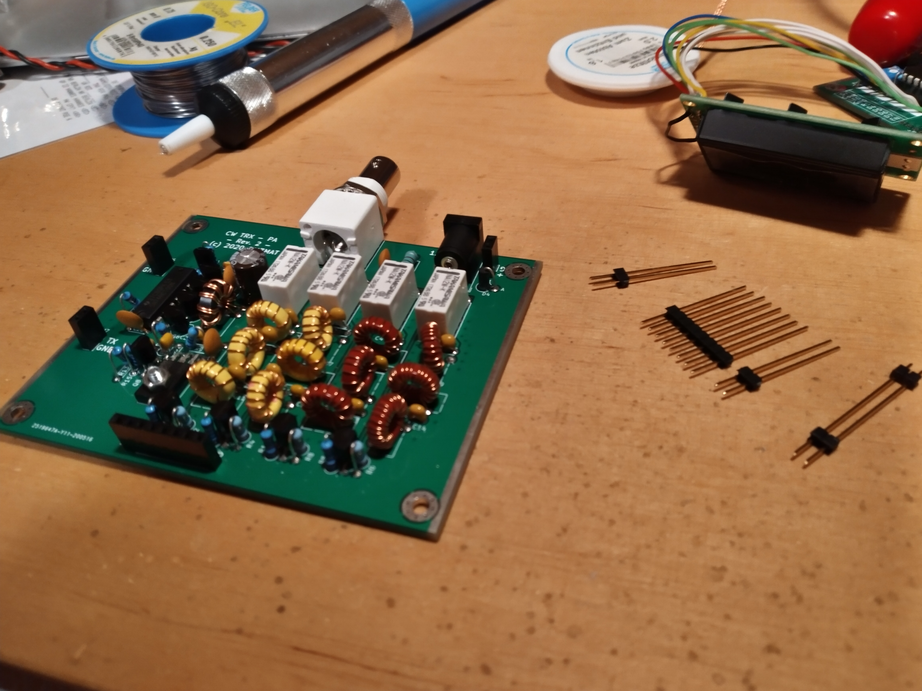
\includegraphics[width=\linewidth]{fig/stackers_small.png}
  \caption{Schneiden Sie das obere Ende der Stapelleisten ab, bevor Sie sie in die Sockel auf der PA Platine stecken.}  \label{fig:stackers}
 \end{subfigure}
 \begin{subfigure}{0.49\linewidth}
  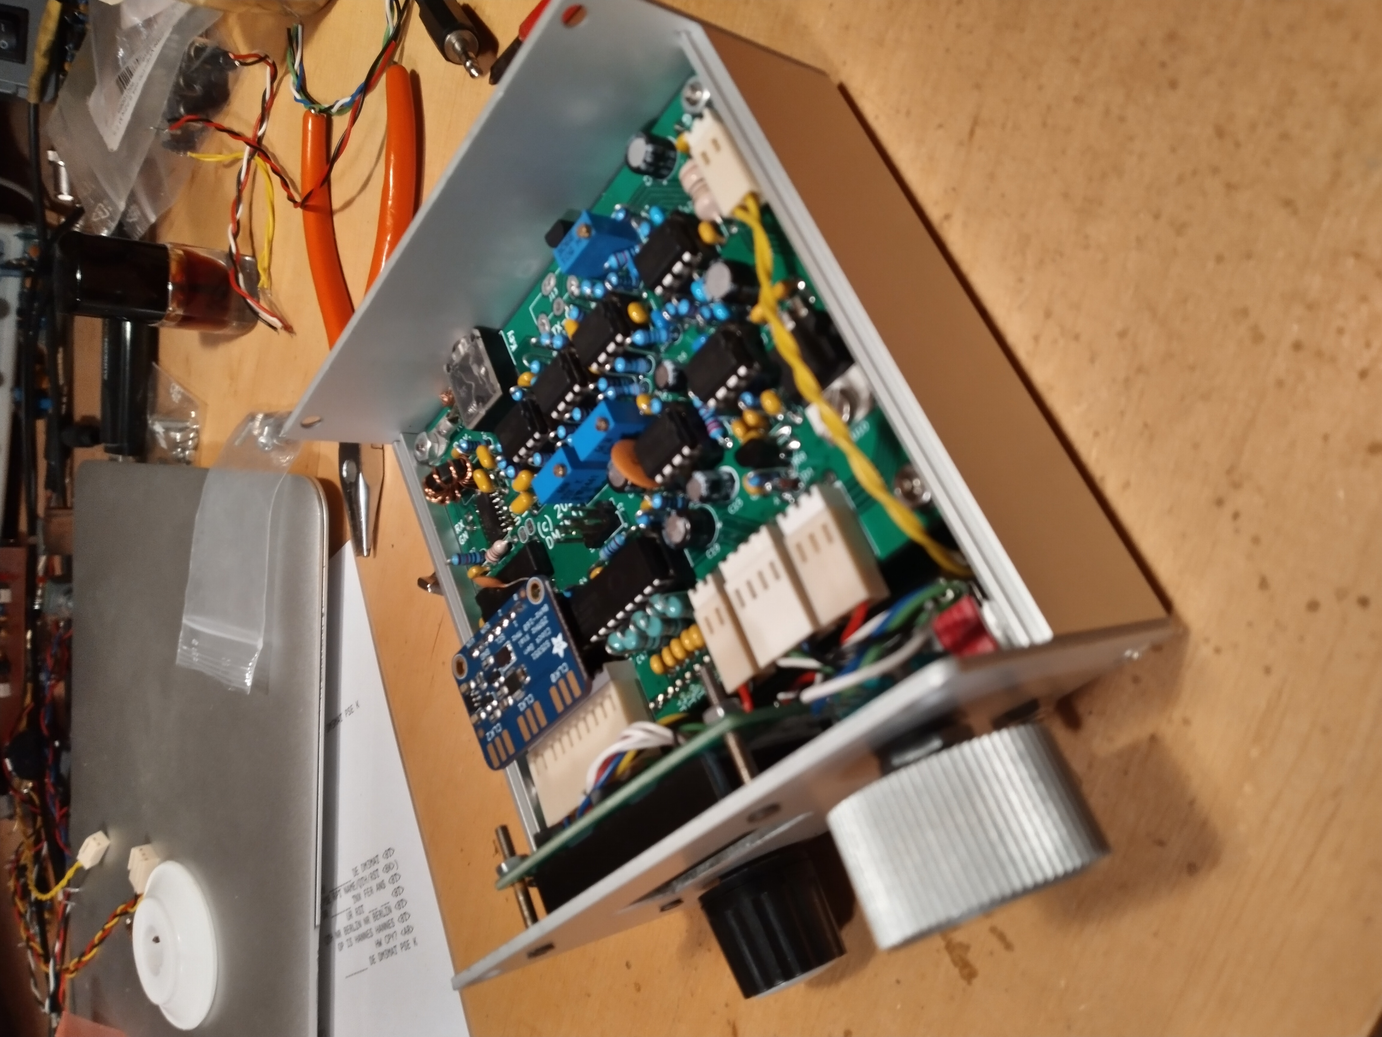
\includegraphics[width=\linewidth]{fig/final_small.png}
  \caption{Stecken Sie die RX Platine auf die Stapelleisten, schieben Sie das Gebilde in die Gehäuseschale, löten Sie die Stapelleisten an der Empfängerplatine fest und schneiden Sie schließlich die Stapelleisten zu.}  \label{fig:final}
 \end{subfigure}
 \caption{Endmontage der Platinen.}
\end{figure}

Der einfachste Weg ist es die oberen Enden der Stapelleisten abzuschneiden (siehe Abbildung \ref{fig:stackers}) und diese dann in die entsprechenden Sockel der PA Platine zu stecken. Führen Sie dann die langen Enden durch die entsprechenden Löcher der RX Platine und schieben Sie beide in das Gehäuse. Löten Sie nun die Stapelleisten auf der RX Platine fest und kürzen Sie die überstehenden Enden.

Wenn Sie das oben erwähnte Fischergehäuse verwenden, wird die RCA Buchse zur Steuerung einer externen PA nicht mehr passen. Die RX und PA Platinen sind einfach zu dicht beieinander. Wenn Sie ein größeres Gehäuse verwenden, können Sie nun die RCA Buchse installieren.


\subsection{Finaler Test}
Mit der abgeschlossenen Endmontage ist es nun an der Zeit die PA und die Sende-Empfangsumschaltung zu testen. Verbinden Sie alles miteinander und schließen Sie ein Dummyload and den Ausgang an. Messen Sie die HF Spannung über dem Dummyload oder schleifen Sie ein HF-Leistungsmeter zwischen TRX und Dummyload ein. Sie sollte etwa $22\,Vp$ oder ca. $5\,W$ am Ausgang messen. Die Leistung hängt auch von der Betriebsspannung ab. Hier werden $13.8\,V$ angenommen.

Wenn Sie deutlich weniger Messen, messen Sie bitte die Spitzenspannungen am PA-Ausgang und Tiefpassfiltereingang. Überprüfen Sie bitte auch nochmals die Tiefpassfilter. Wenn alles zu Ihrer Zufriedenheit ist, ist der Aufbau abgeschlossen.

\subsection{Hot fixes}
Die zweite Revision war beinahe ein Redesign. Daher ist noch nicht alles Perfekt. Zum Beispiel produziert der \texttt{74AC74} recht hohe Hochfrequenzspannungen auf der $5\,V$ Spannungsversorgung. Um diese stärker zu dämpfen löten Sie bitte einen $470\,pF$ Kondensator direkt von Pin 16 (5V) zu Pin 8 (GND).

Die Audioendstufe neigt leider zum Schwingen, vor allem wenn ein kleiner Lautsprecher verwendet wird. Wenn das passiert, wird der gesamte Audiopfad in die Sättigung getrieben. Dabei kann bis zu 12V an den Mixer geführt werden, was diesen dann zerstört! Um das zu verhindern, \textbf{sollten} vier 5.1V Zenerdioden parallel zu den Kondensatoren C4-C7 auf dem RX-Board fliegend gelötet werden. 

\clearpage
\subsection{Mechanical Parts}
\begin{longtable}{|l|p{6cm}|l|l|} \hline 
\# & Component & Remarks \\ \hline 
1 & chassis top & \\
1 & chassis bottom & \\
1 & chassis front/back & \\
1 & 10k log pot & \\
1 & rotary encoder & \\
1 & LCD display & \\
1 & head-phone socket & \\
1 & switch & \\
1 & barrel plug & \\
2 & fuse holder & optional \\
2 & 2A flink & optional \\
1 & speaker & optional \\ \hline
\end{longtable}


\cleardoublepage
\section{Bedienung} \label{sec:user}
Einen komplexen TRX mit einem Drehimpulsgeber zu bedienen ist recht schwierig. Ich habe daher ein zwei-ebenen Menu entworfen, dass alles Wichtige in die erste Ebene (blau in Abb. \ref{fig:menu}) und alles weniger Wichtige in die Zweite ebene (rot in Abb. \ref{fig:menu}) verbannt. Das erlaubt eine schnelle Handhabung für häufig verwendete Menüpunkte.

\begin{figure}[!ht]
 \centering
 \footnotesize
 \begin{tikzpicture}[node distance=2.3cm,
	>={Latex[width=2mm,length=2mm]},
    menu/.style = {rectangle, rounded corners, draw=black,
                   minimum width=1.5cm, minimum height=1cm,
                   text centered, font=\sffamily, fill=blue!30},
    submenu/.style = {menu, fill=red!30}]
  \node (rit) [menu] {RIT};   
  \node (speed) [menu, right of=rit] {CW Speed}; 
  \node (step) [menu, right of=speed]{Step size};
  \node (vfo) [menu, right of=step] {VFO};
  \node (band) [menu, right of=vfo] {Band};
  \node (setup) [menu, right of=band] {Setup};
  
  \node (quick) [submenu, below of=setup] {Qick-set};
  \node (cw) [submenu, left of=quick] {CW Mode}; 
  \node (tone) [submenu, left of=cw] {CW Tone}; 
  \node (level) [submenu, left of=tone] {CW Level}; 
  \node (text) [submenu, left of=level] {CW Text}; 
  \node (clr) [submenu, left of=text] {Clr. CWT};
  \node (meter) [submenu, below of=clr] {Meter};
  \node (hold) [submenu, below of=meter] {TX Hold}; 
  \node (greet) [submenu, right of=hold] {Greet};
  \node (enc) [submenu, right of=greet] {Enc.Type};
  \node (version) [submenu, right of=enc] {Version};
  \node (sideband) [submenu, right of=version] {USB/LSB};
  \node (pll) [submenu, right of=sideband] {PLL Cor.};
  \node (reset) [submenu, above of=pll] {Reset};
  
  
  \path[->,thick]
    (rit) edge (speed)
    (speed) edge (step)
	(step) edge (vfo)
	(vfo) edge (band)
	(band) edge (setup)
	(setup) edge[bend right] (rit);
	
  \path[->,thick,dashed]
    (setup) edge (quick);
  \path[->,thick]
        (quick) edge (cw)
    	(cw) edge (tone)
    	(tone) edge (level) 
    	(level) edge (text)
    	(text) edge (clr)
    	(clr) edge (meter) 
    	(meter) edge (hold)
    	(hold) edge (greet) 
    	(greet) edge (enc)
    	(enc) edge (version)
    	(version) edge (sideband)
    	(sideband) edge (pll)
    	(pll) edge (reset) 
    	(reset) edge (quick);
 \end{tikzpicture}
 \caption{Menu navigation} \label{fig:menu}
\end{figure}

Um in das Menu zu gelangen, drücken Sie einfach kurz auf den Achsentaster des Impulsgebers. Sie werden dann auf der RIT Einstellung oder der zuletzt verwendeten Einstellung landen. Drehen Sie nun den Impulsgeber um in der ersten Ebene des Menüs zu navigieren. Um eine Einstellung zu ändern, drücken Sie nochmals kurz auf den Achsentaster. Sie können nun die ausgewählte Einstellung ändern. Um die Änderung zu speichern und das Menü zu verlassen, drücken Sie nochmals kurz auf den Achsentaster.

Um die zweite Menüebene zu erreichen, drücken Sie zunächst kurz auf den Achsentaster um in die erste Ebene zu gelangen. Wählen Sie dann den Menüpunkt \texttt{Setup} aus und drücken Sie nochmals kurz den Achsentaster. Sie befinden sich nun in der zweiten Menüebene. Das Navigieren, Bearbeiten und Verlassen der zweiten Ebene erfolgt genauso wie in der ersten Menüebene.

\subsection{Gesten}
Die Firmware unterscheidet zwischen 4 verschiedenen \emph{Gesten} den Sie mit dem Drehimpulsgeber ausführen können:
\begin{enumerate}
 \item \emph{drehen} - Einfach den Impulsgeber drehen.
 \item \emph{klick} - Kurzes drücken und wieder loslassen des Achsentasters.
 \item \emph{gedrückt halten} - Langes (mind. $2\,s$) gedrückt halten des Achsentasters.
 \item \emph{drücken \& drehen} - Halten die den Achsentaster gedrückt und drehen Sie gleichzeitig den Impulsgeber.
\end{enumerate}

Während des Empfangs wird durch die \emph{drehen} Geste die Frequenz eingestellt (natürlich), eine \emph{klick} Geste wird das Menü öffnen, die \emph{gedrückt halten} Geste wird den gespeicherten Text senden (falls konfiguriert) und die \emph{drücken \& drehen} Geste wird die sogenannte \emph{quick-set} Einstellung ändern (falls konfiguriert).


\subsection{Einstellungen}
Als \emph{Einstellungen} wird alles Bezeichnet, was während des Betriebs geändert werden kann. Diese Einstellungen sind daher auch alle in der ersten Menüebene zu finden. 
 
\paragraph{Receive/Transmit offset (RIT)}
Erlaubt es die Empfangsfrequenz relativ zur Sendefrequenz zu verstimmen. Eine von null verschiedene RIT wird durch ein \texttt{+} oder \texttt{-} Symbol in der rechten unteren Ecke angezeigt.

\paragraph{CW speed}
Die Gebegeschwindigkeit in WPM.

\paragraph{Tuning step-size}
Die Abstimmschrittweite.

\paragraph{VFO}
Der aktuelle VFO. Entweder \texttt{VFO A}, \texttt{VFO B} oder \texttt{Split}.

\paragraph{Band}
Das aktuelle Band.


\subsection{Setup}
Im \emph{Setup} werden alle Einstellungen versteckt, die üblicherweise nicht während des Betriebs geändert werden. Sie sind daher in die zweite Menüebene verband.

\paragraph{Quick-set}
Das \emph{quick-set} Feature erlaubt es Ihnen eine bestimmte Einstellung (siehe oben) während des Empfangs zu ändern ohne dazu erst das Menü aufrufen zu müssen. Hier können Sie diese Einstellung auswählen: RIT, Gebegeschwindigkeit, Schrittweite, Band oder eben \texttt{none}. Letzteres deaktiviert \emph{quick-set}.

\paragraph{Keyer mode}
Stellt die Art der Taste ein. Entweder \emph{straight key} oder \emph{iambic}.

\paragraph{CW side-tone level}
Stellt die Lautstärke des CW Seitentons ein. Dies ist ein Wert zwischen 1 und 255.

\paragraph{Keyer memory \texttt{CW Text}}
Legt den Text fest, der gesendet wird, wenn der Achsentaster lange gedrückt wird. Wenn kein Text gespeichert ist wird nichts passieren.

Um den Text zu editieren drücken sie nun kurz den Achsentaster. Sie sollten nun einen Kursor unter dem ersten Zeichen des Textes sehen. Wenn Sie nun am Impulsgeber drehen, können Sie das Zeichen auswählen, das sie editieren wollen. Drücken sie nochmals kurz den Achsentaster um das ausgewählte Zeichen zu ändern. Das gewählte Zeichen sollte nun blinken. Wenn die das Zeichen geändert haben drücken Sie nochmals kurz auf den Achsentaster. Der Kursor sollte nun eine Stelle weiter gesprungen sein. Fahren Sie nun so fort bis der gewünschte Text erstellt ist (z.B. ein CQ Ruf). Um den Text zu speichern und das Menu zu verlassen, drücken und halten Sie den Achsentaster für mindestens 2 Sekunden.

\paragraph{Clear keyer memory}
Dieser Menüpunkt löscht den gespeicherten Text.

\paragraph{Meter selection}
Wählt die Anzeige während des Empfangs aus. Dies kann \texttt{Volt}, \texttt{Temp} oder \texttt{None} sein. Wenn Sie \texttt{Volt} wählen wird die Versorgungsspannung kontinuierlich gemessen und angezeigt. Wenn Sie \texttt{Temp} wählen wird die Kerntemperatur der MCU gemessen und angezeigt. Wenn Sie \texttt{None} gewählt haben, wird nichts angezeigt.

\paragraph{TX-hold time}
Legt die Länge der Umschaltpause im $ms$ fest. Standardmäßig ist sie auf $50\,ms$ festgelegt. Dieser kleine Wert erlaubt quasi-QSK. 
\begin{remark}
Wenn Sie eine externe PA verwenden oder im Split Modus operieren, sollten Sie eine längere Umschaltpause wählen um den Relais genügend Zeit um Umschalten zu gewähren.
\end{remark}

\paragraph{Greet text}
Dieser Editor erlaubt es den Begrüßungstext beim booten zu ändern. Dieser Editor funktioniert genau so wie der CW-Texteditor.

\paragraph{CW Seitenton}
Stellt die Frequenz des CW Seitentons ein. Diese Frequenz legt auch den Shift zwischen der Sende und Empfangsfrequenz fest und sollte daher der Mittenfrequenz des CW Audiofilters ($\approx 700\,Hz$) entsprechen.

\paragraph{Encoder type}
Legt den Typ des Drehimpulsgebers fest. Es gibt zwei verbreitete Typen \texttt{A} \& \texttt{B}. Wenn Sie genau den Encoder aus der BOM bestellt haben, haben Sie Typ A. Wenn Sie Probleme mit dem Encoder haben (Doppelschritte), sollten Sie hier Typ B einstellen.

\paragraph{PLL correction}
Diese Einstellung legt die PLL Frequenzkorrektur in PPM fest.

\paragraph{Factory reset}
Vorherige Versionen hatten einige Probleme mit korrumpierten EEPROM Speicher. Dieser Menüpunkt erlaubt es Ihnen den EEPROM auf den Auslieferungszustand zurückzusetzen.


\cleardoublepage
\section{Bill-of-Material (BOM)}
\begin{longtable}{|p{0.02\textwidth}|p{0.02\textwidth}|p{0.3\textwidth}|p{0.3\textwidth}|p{0.07\textwidth}|p{0.07\textwidth}|}\hline
\# & & Value & Reichelt & Cost & Sum \\ \hline\hline
1 & $\square$ & 10R & METALL 10,0 & 0,05 \euro & 0,05 \euro \\
6 & $\square$ & 100R & METALL 100 & 0,05 \euro & 0,29 \euro \\
1 & $\square$ & 220R & METALL 220 & 0,05 \euro & 0,05 \euro \\ 
1 & $\square$ & 470R & METALL 470 & 0,05 \euro & 0,05 \euro \\
4 & $\square$ & 1k & METALL 1,00K & 0,05 \euro & 0,20 \euro \\
1 & $\square$ & 2.2k & METALL 2,20K & 0,05 \euro & 0,05 \euro \\
9 & $\square$ & 3.3k & METALL 3,30K & 0,05 \euro & 0,44 \euro \\
1 & $\square$ & 4.3k & METALL 4,30K & 0,05 \euro & 0,05 \euro \\
2 & $\square$ & 4.7k & METALL 4,70K & 0,05 \euro & 0,10 \euro \\
1 & $\square$ & 5.1k & METALL 5,10K & 0,05 \euro & 0,05 \euro \\
1 & $\square$ & 7.5k & METALL 7,50K & 0,05 \euro & 0,05 \euro \\
17 & $\square$ & 10k & METALL 10,0K & 0,05 \euro & 0,83 \euro \\
2 & $\square$ & 30k & METALL 30,0K & 0,05 \euro & 0,10 \euro \\
2 & $\square$ & 33k & METALL 33,0K & 0,05 \euro & 0,10 \euro \\
2 & $\square$ & 36k & METALL 36,0K & 0,05 \euro & 0,10 \euro \\
2 & $\square$ & 47k & METALL 47,0K & 0,05 \euro & 0,10 \euro \\
4 & $\square$ & 100k & METALL 100K & 0,05 \euro & 0,20 \euro \\
1 & $\square$ & 120k & METALL 120K & 0,05 \euro & 0,05 \euro \\
1 & $\square$ & 470k & METALL 470K & 0,05 \euro & 0,05 \euro \\
2 & $\square$ & 50k & 64W-50K & 0,31 \euro & 0,62 \euro \\
1 & $\square$ & 500R & 64W-500 & 0,27 \euro & 0,27 \euro \\
1 & $\square$ & 10k & ACP 6-L 10K & 0,21 \euro & 0,21 \euro \\ \hline
2 & $\square$ & 100p & NPO-2,5 100P & 0,07 \euro & 0,14 \euro \\
4 & $\square$ & 220p & NPO-2,5 220P & 0,08 \euro & 0,32 \euro \\
4 & $\square$ & 470p & NPO-2,5 470P & 0,09 \euro & 0,36 \euro \\
2 & $\square$ & 820p & Conrad: 1578706 & 0,16 \euro & 0,32 \euro \\
3 & $\square$ & 1n & X7R-2,5 1,0N & 0,07 \euro & 0,21 \euro \\
2 & $\square$ & 1n & NPO-2,5 1,0N & 0,09 \euro & 0,18 \euro \\
2 & $\square$ & 1.5n & X7R-2,5 1,5N & 0,07 \euro & 0,14 \euro \\
2 & $\square$ & 3.3n & X7R-2,5 3,3N & 0,07 \euro & 0,14 \euro \\
3 & $\square$ & 10n & X7R-2,5 10N & 0,07 \euro & 0,21 \euro \\
5 & $\square$ & 47n & X7R-2,5 47N & 0,11 \euro & 0,55 \euro \\
35 & $\square$ & 100n & Z5U-2,5 100N & 0,05 \euro & 1,75 \euro \\
5 & $\square$ & 470n & Z5U-5 470N & 0,19 \euro & 0,95 \euro \\
3 & $\square$ & 1u & Z5U-5 1,0µ & 0,26 \euro & 0,78 \euro \\ \hline		
3 & $\square$ & 10u & RAD 10/35 & 0,02 \euro & 0,06 \euro \\
3 & $\square$ & 100u & RAD 100/16 & 0,03 \euro & 0,09 \euro \\
1 & $\square$ & 220u & RND 150ECR AY & 0,06 \euro & 0,06 \euro \\ \hline
1 & $\square$ & 22u & L-07HCP 22µ & 0,38 \euro & 0,38 \euro \\
9 & $\square$ & 100u & L-MICC 100µ & 0,27 \euro & 2,43 \euro \\ \hline
2 & $\square$ & FT37-43 & FT 37-43 & 0,58 \euro & 1,16 \euro \\
6 & $\square$ & T 37-6 & T 37-6 & 0,78 \euro & 4,68 \euro \\
6 & $\square$ & T 37-2 & T 37-2 & 0,54 \euro & 3,24 \euro \\ \hline
7 & $\square$ & 1N4148 & 1N 4148 & 0,02 \euro & 0,14 \euro \\
1 & $\square$ & 1N4001 & 1N 4001 & 0,02 \euro & 0,02 \euro \\
4 & $\square$ & 5.1V Zener & RND 1N751A &0,02 \euro & 0,08 \euro \\
7 & $\square$ & BS170 & BS 170 & 0,10 \euro & 0,70 \euro \\
5 & $\square$ & 2N3904 & 2N 3904 & 0,04 \euro & 0,20 \euro \\
1 & $\square$ & BD140 & BD 140-16 STM & 0,19 \euro & 0,19 \euro \\
1 & $\square$ & FST3253 & SOIC-16, Ebay & 2,00 \euro & 2,00 \euro \\
5 & $\square$ & LM833 & LM 833 & 0,90 \euro & 4,50 \euro \\
1 & $\square$ & LM386 & LM 386 DIP & 0,22 \euro & 0,22 \euro \\
6 & $\square$ & DIP-8 socket (optional) & GS 8 & 0,04 \euro & 0,24 \euro \\
1 & $\square$ & 74AC74 & Kessler: 522421 & 0,36 \euro & 0,36 \euro \\
1 & $\square$ & 74HCT00 & 74HCT 00 & 0,33 \euro & 0,33 \euro \\
1 & $\square$ & L7805 & L 7805 CV & 0,25 \euro & 0,25 \euro \\
1 & $\square$ & ATmega328-PU & ATMEGA 328P-PU & 2,50 \euro & 2,50 \euro \\
1 & $\square$ & DIP-28 socket (optional) & GS 28-S & 0,10 \euro & 0,10 \euro \\
1 & $\square$ & SI5351 breakout & Adafruit & 7,35 \euro & 7,35 \euro \\ \hline
4 & $\square$ & G6S-2 & NA 12W K & 0,96 \euro & 3,84 \euro \\ \hline
2 & $\square$ & 1x10 pin-header long & STAPELLEISTE 10 & 0,38 \euro & 0,76 \euro \\
1 & $\square$ & 2x3 pin-header & MPE 087-2-006 & 0,14 \euro & 0,14 \euro \\
1 & $\square$ & 1x7 pin-socket & MPE 156-1-007 & 0,37 \euro & 0,27 \euro \\
2 & $\square$ & 1x2 90deg & PSS 254/2W & 0,02 \euro & 0,04 \euro \\
2 & $\square$ & 1x2 plug & PSK 254/2W & 0,02 \euro & 0,04 \euro \\
1 & $\square$ & 1x3 90deg & PSS 254/3W & 0,04 \euro & 0,04 \euro \\
1 & $\square$ & 1x3 plug & PSK 254/3W & 0,02 \euro & 0,02 \euro \\
1 & $\square$ & 1x4 90deg & PSS 254/4W & 0,09 \euro & 0,09 \euro \\
1 & $\square$ & 1x4 plug & PSK 254/4W & 0,02 \euro & 0,02 \euro \\
1 & $\square$ & 1x10 90deg & PSS 254/10W & 0,10 \euro & 0,10 \euro \\
1 & $\square$ & 1x10 plug & PSK 254/10W & 0,08 \euro & 0,08 \euro \\
2 & $\square$ & contacts & PSK-KONTAKTE & 0,29 \euro & 0,58 \euro \\
2 & $\square$ & head-phone socket & EBS 35 & 0,30 \euro & 0,60 \euro\\
1 & $\square$ & TX-OC & CBP & 0,21 \euro & 0,21 \euro \\
1 & $\square$ & BNC & UG 1094W1 & 0,99 \euro & 0,99 \euro \\
1 & $\square$ & 1 x 8 socket & MPE 094-1-008 & 0,24 \euro & 0,14 \euro \\
1 & $\square$ & barrel jack & DC BU21 90 & 0,46 \euro & 0,46 \euro \\
3 & $\square$ & 1 x 2 socket & RND 205-00642 & 0,02 \euro & 0,06 \euro \\ \hline
1 & $\square$ & chassis top & KOH-2100 & 5,40 \euro & 5,40 \euro \\
1 & $\square$ & chassis bottom & KOH-4100 & 5,80 \euro & 5,80 \euro \\
1 & $\square$ & chassis front/back & DPL 2-4 & 7,99 \euro & 7,99 \euro \\
1 & $\square$ & 10k log pot & RK11K112-LOG10K & 1,35 \euro & 1,35 \euro \\
1 & $\square$ & rotary encoder & STEC11B03 & 3,70 \euro & 3,70 \euro \\
1 & $\square$ & LCD display & LCD-PM 2X8-5 A & 7,30 \euro & 7,30 \euro \\
1 & $\square$ & switch & KIPP 1A11 & 1,20 \euro & 1,20 \euro \\
1 & $\square$ & barrel plug & HS 21-13 & 0,20 \euro & 0,20 \euro \\
2 & $\square$ & fuse holder (optional) & RND 170-00170 & 0,19 \euro & 0,38 \euro \\
2 & $\square$ & 2A flink (optional) & ESKA 520.020 & 0,09 \euro & 0,18 \euro \\
1 & $\square$ & speaker (optional) & LSM-S20K & 2,70 \euro & 2,70 \euro \\ \hline \hline
\multicolumn{4}{|l}{Total\footnote{Prices may change over time.}} & \multicolumn{2}{r|}{\textbf{89,21 \euro}} \\ \hline
\end{longtable}


\subsection{Ein paar \euro\ sparen}
Der teuerste Einzelposten auf der BOM ist das Gehäuse. Sie können sicher ein Alugehäuse für unter \EUR{5} bei ebay finden. Sie finden auch billige Clone der SI5351 break-out Platine für um die \EUR{3}, billige Drehimpulsgeber und 2x8 LCD Displays dort. So können Sie die BOM Kosten noch deutlich senken.

\cleardoublepage
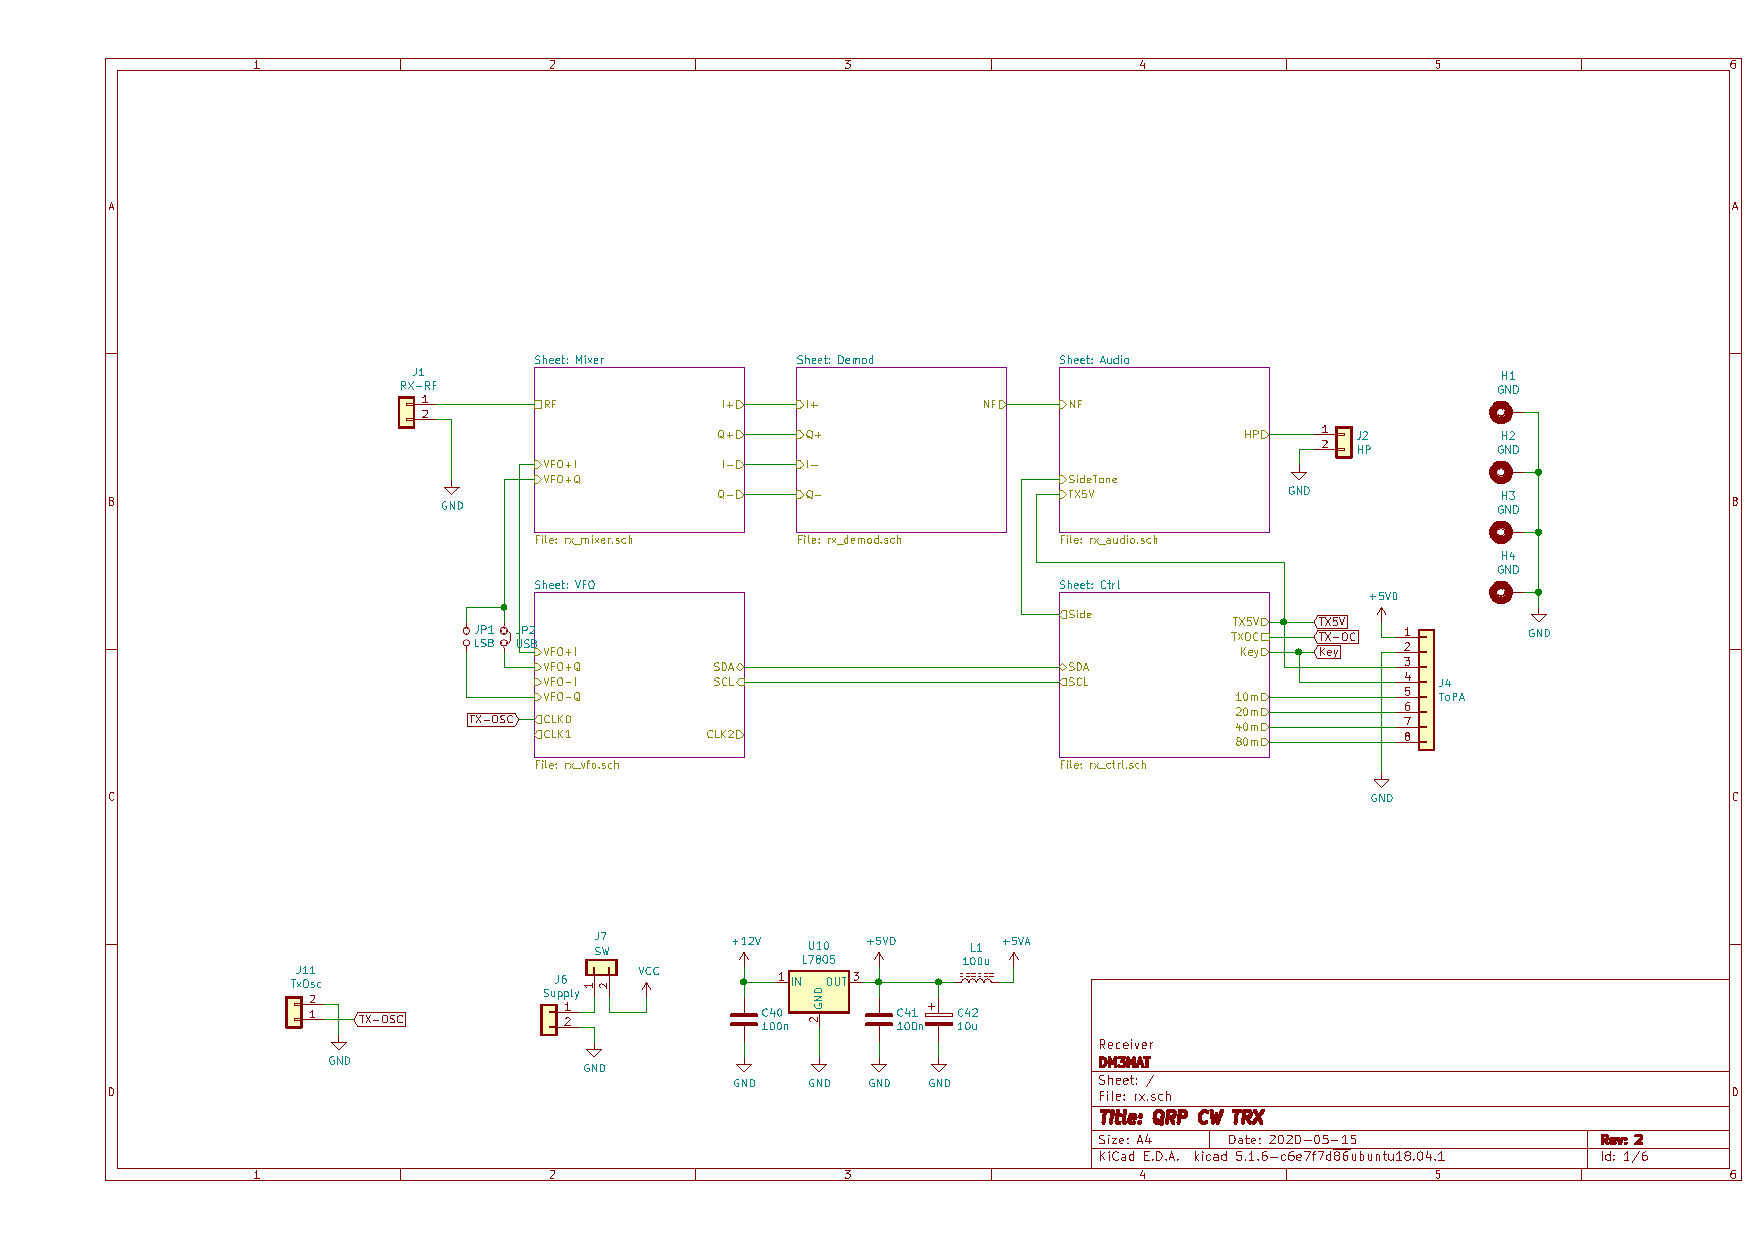
\includepdf[pages={1,2,4,3,5,6},landscape=true, addtotoc={
 1, section, 1, RX Circuit, rxscm,
 2, subsection, 1, RX Mixer, rxmix,
 4, subsection, 1, Demodulator, rxdemod,
 3, subsection, 1, AF-Section, rxaudio,
 5, subsection, 1, PLL, rxpll,
 6, subsection, 1, Controller, rxctrl}]{fig/rx_scm.pdf}
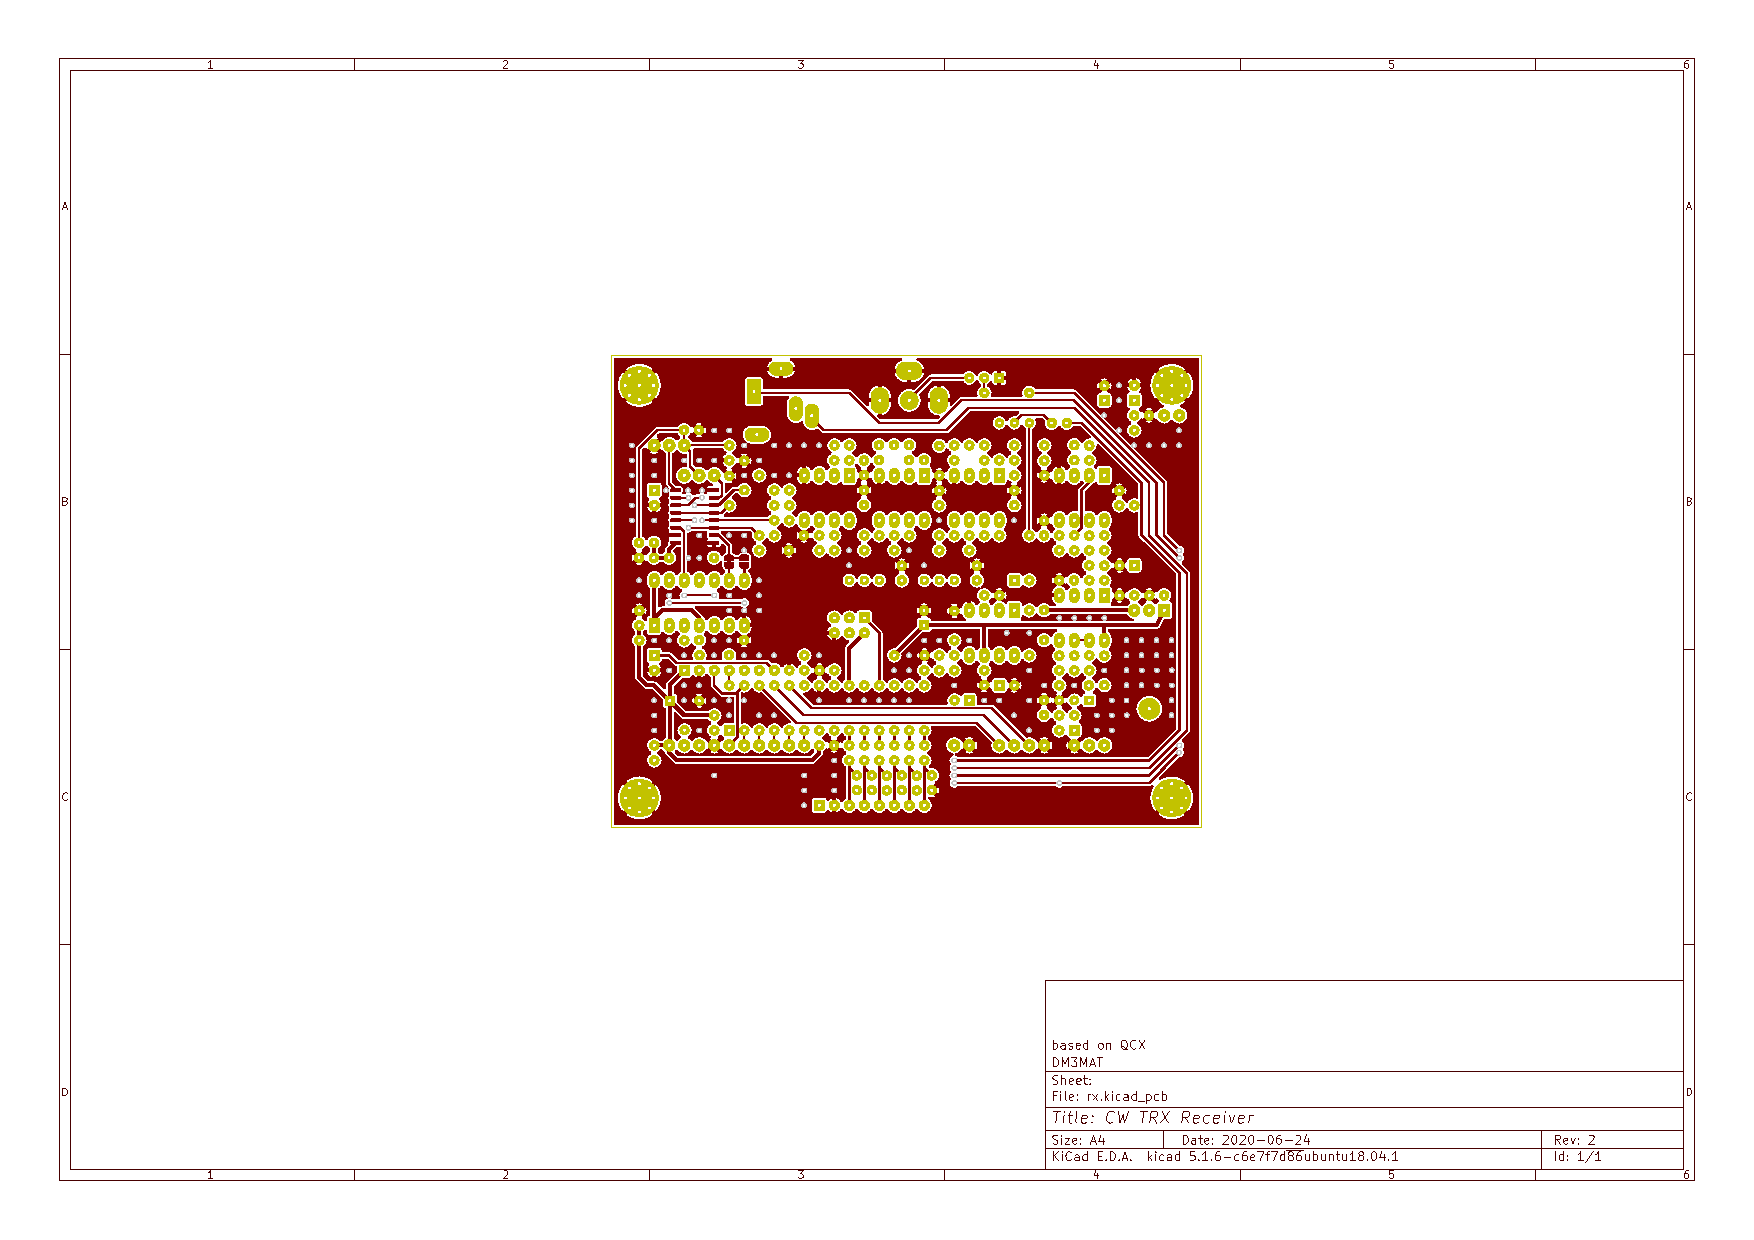
\includepdf[pages={1,2,3},landscape=true, addtotoc={
 1, section, 1, RX Board, rxbrdtop,
 2, subsection, 1, Bottom, rxbrdbottom,
 3, subsection, 1, Silkscreen, rxbrdsilk}]{fig/rx_brd.pdf}
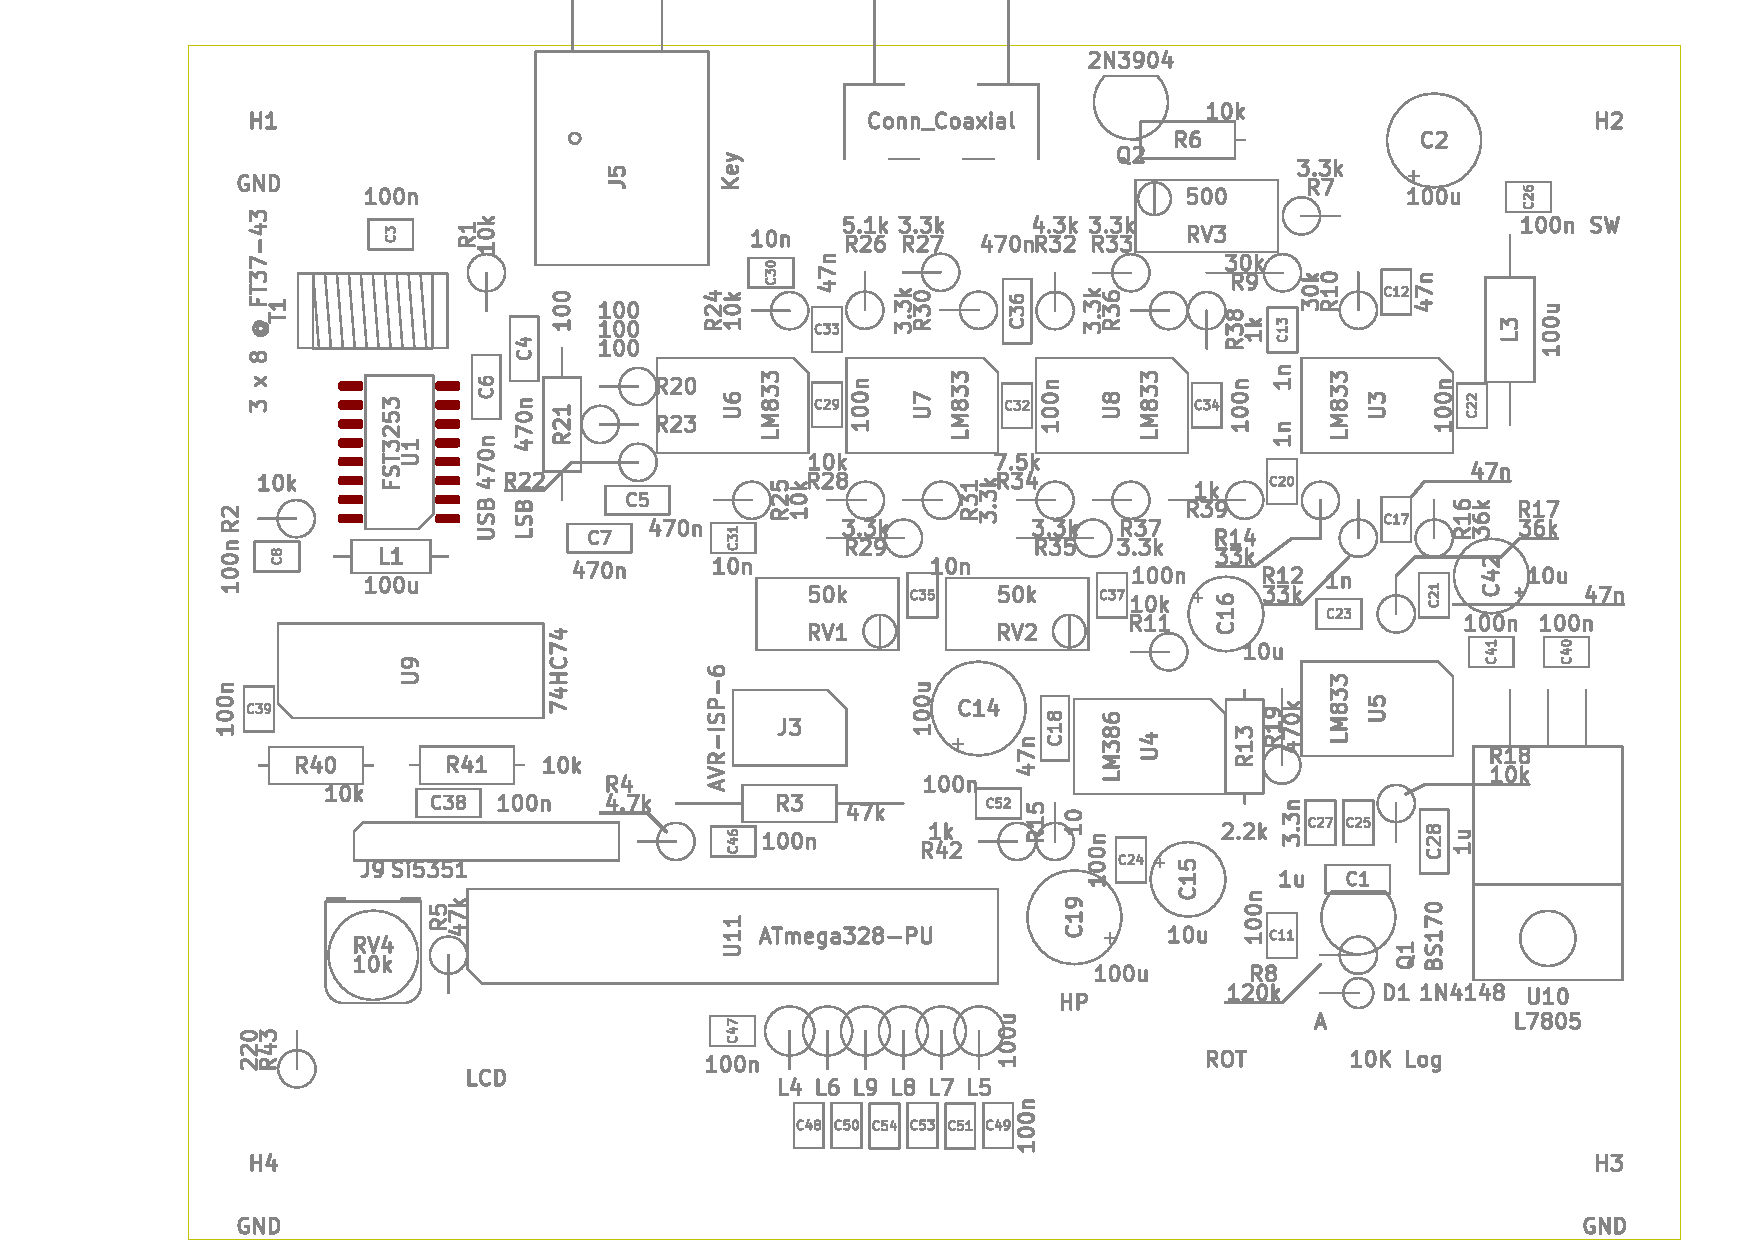
\includepdf[landscape=true, addtotoc={
 1, subsection, 1, Component Placement \& Values, rxval}]{fig/rx_values.pdf}
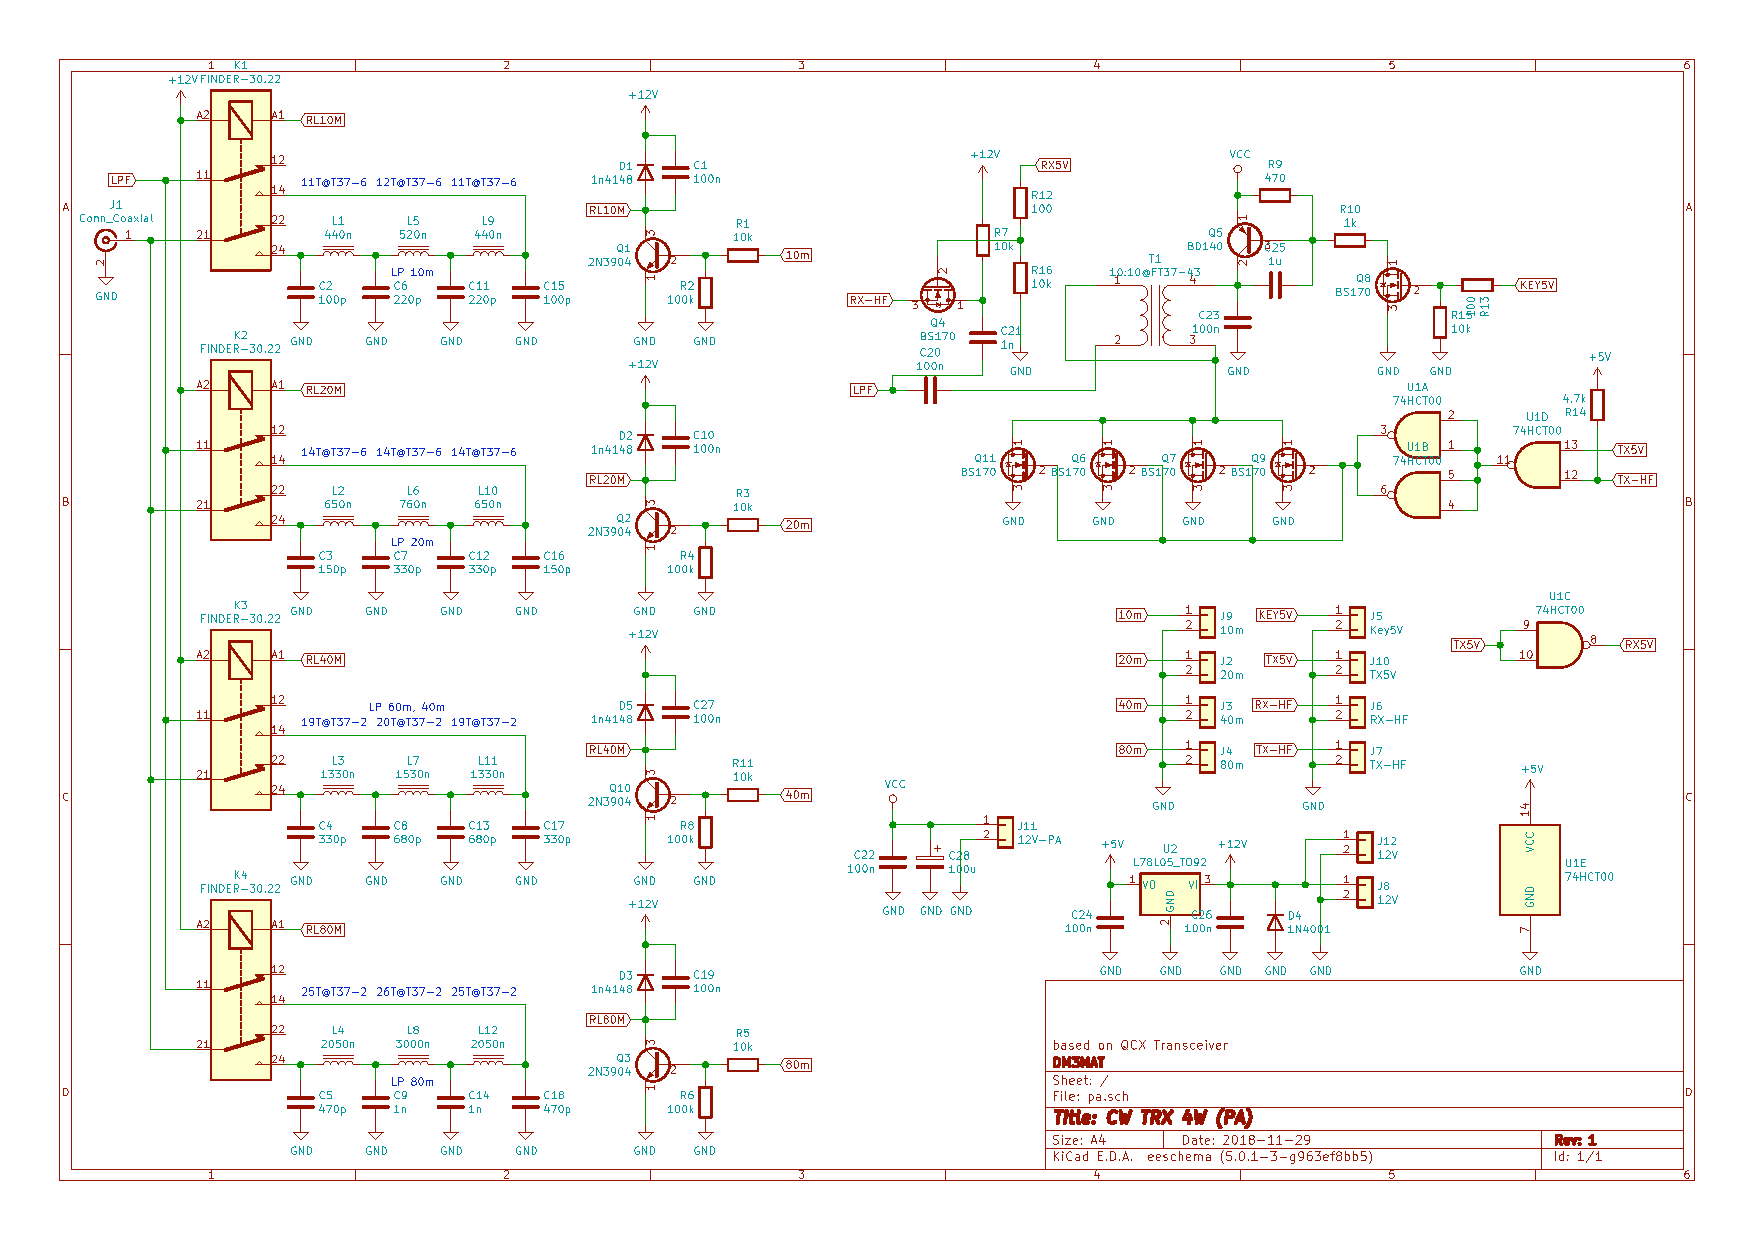
\includepdf[landscape=true, addtotoc={
 1, section, 1, PA/LP Circuit, pascm}]{fig/pa_scm.pdf}
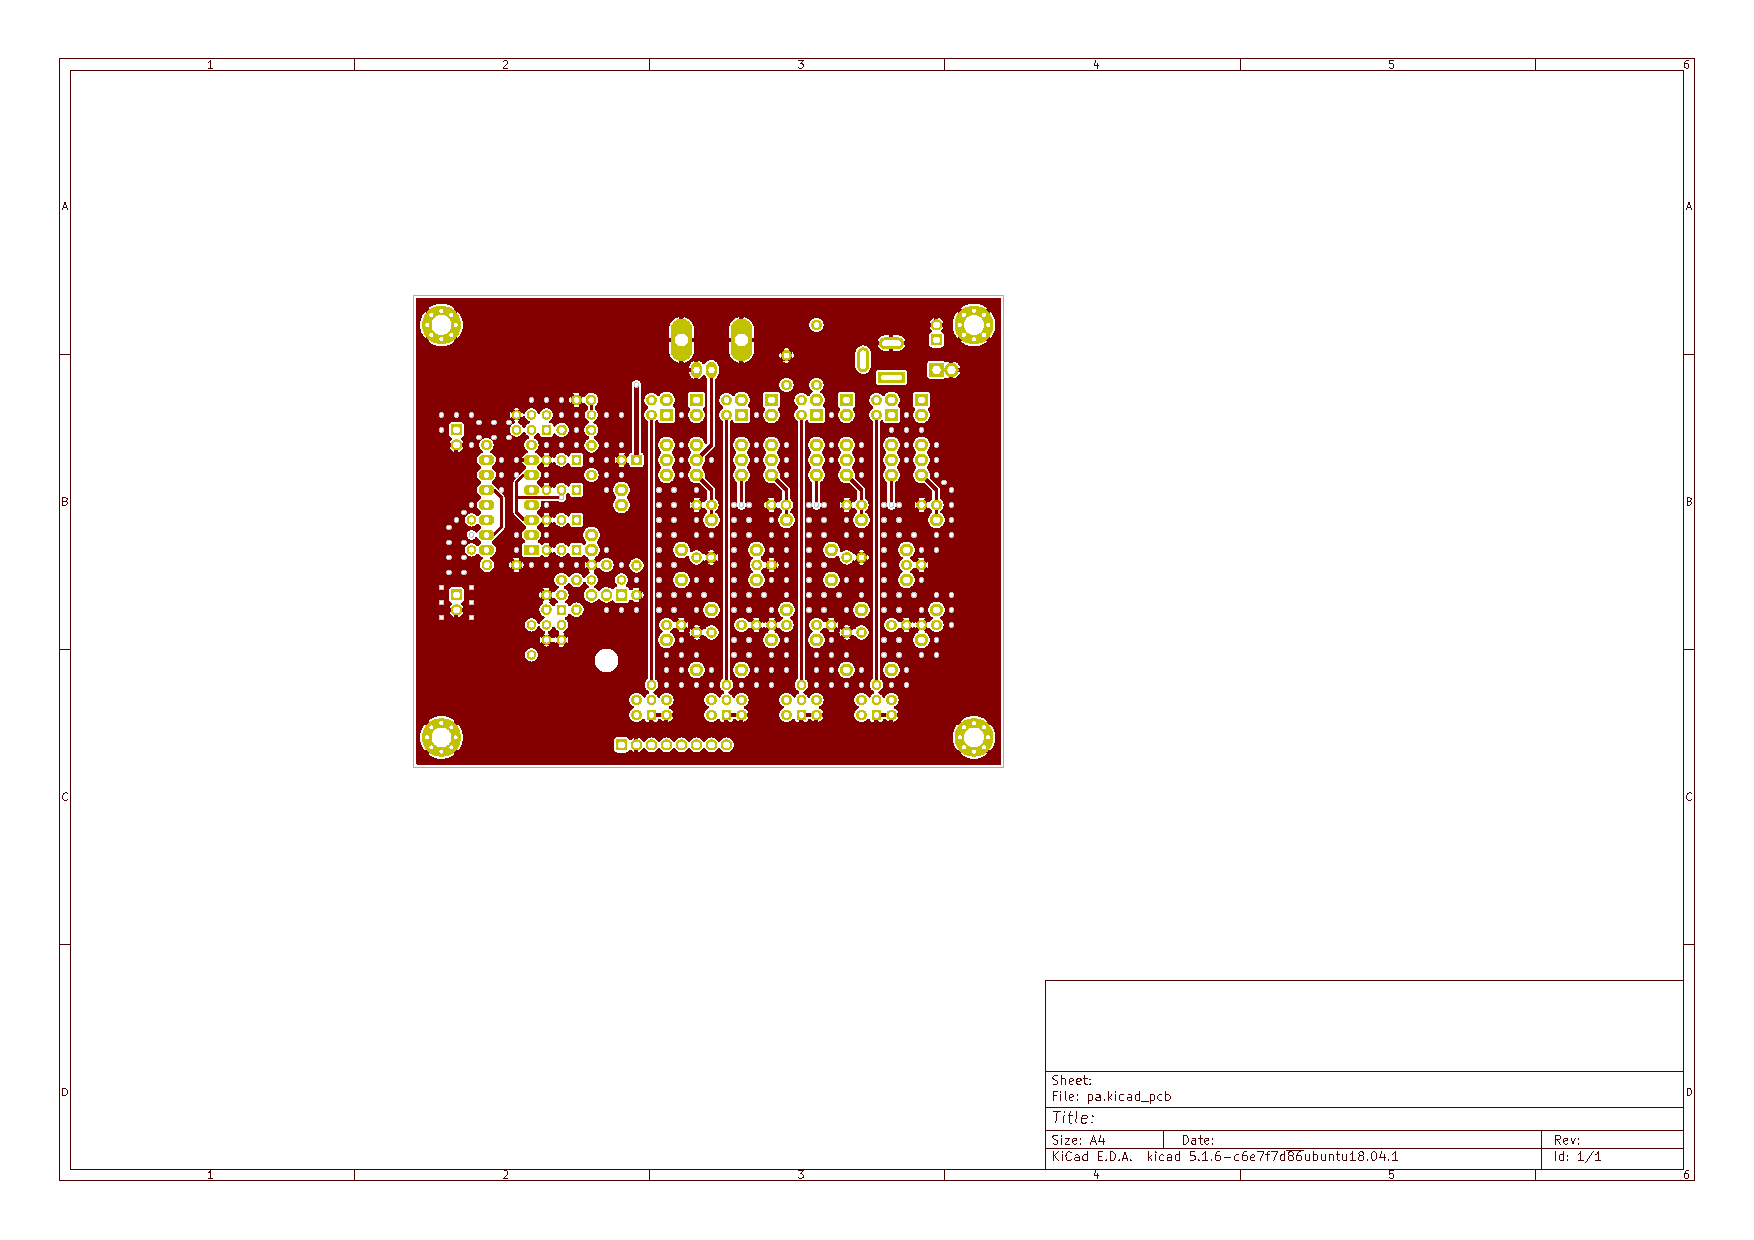
\includepdf[pages={1,2,3},landscape=true, addtotoc={
 1, section, 1, PA/LP Board, pabrdtop,
 2, subsection, 1, Bottom, pabrdbottom,
 3, subsection, 1, Silkscreen, pabrdsilk}]{fig/pa_brd.pdf}
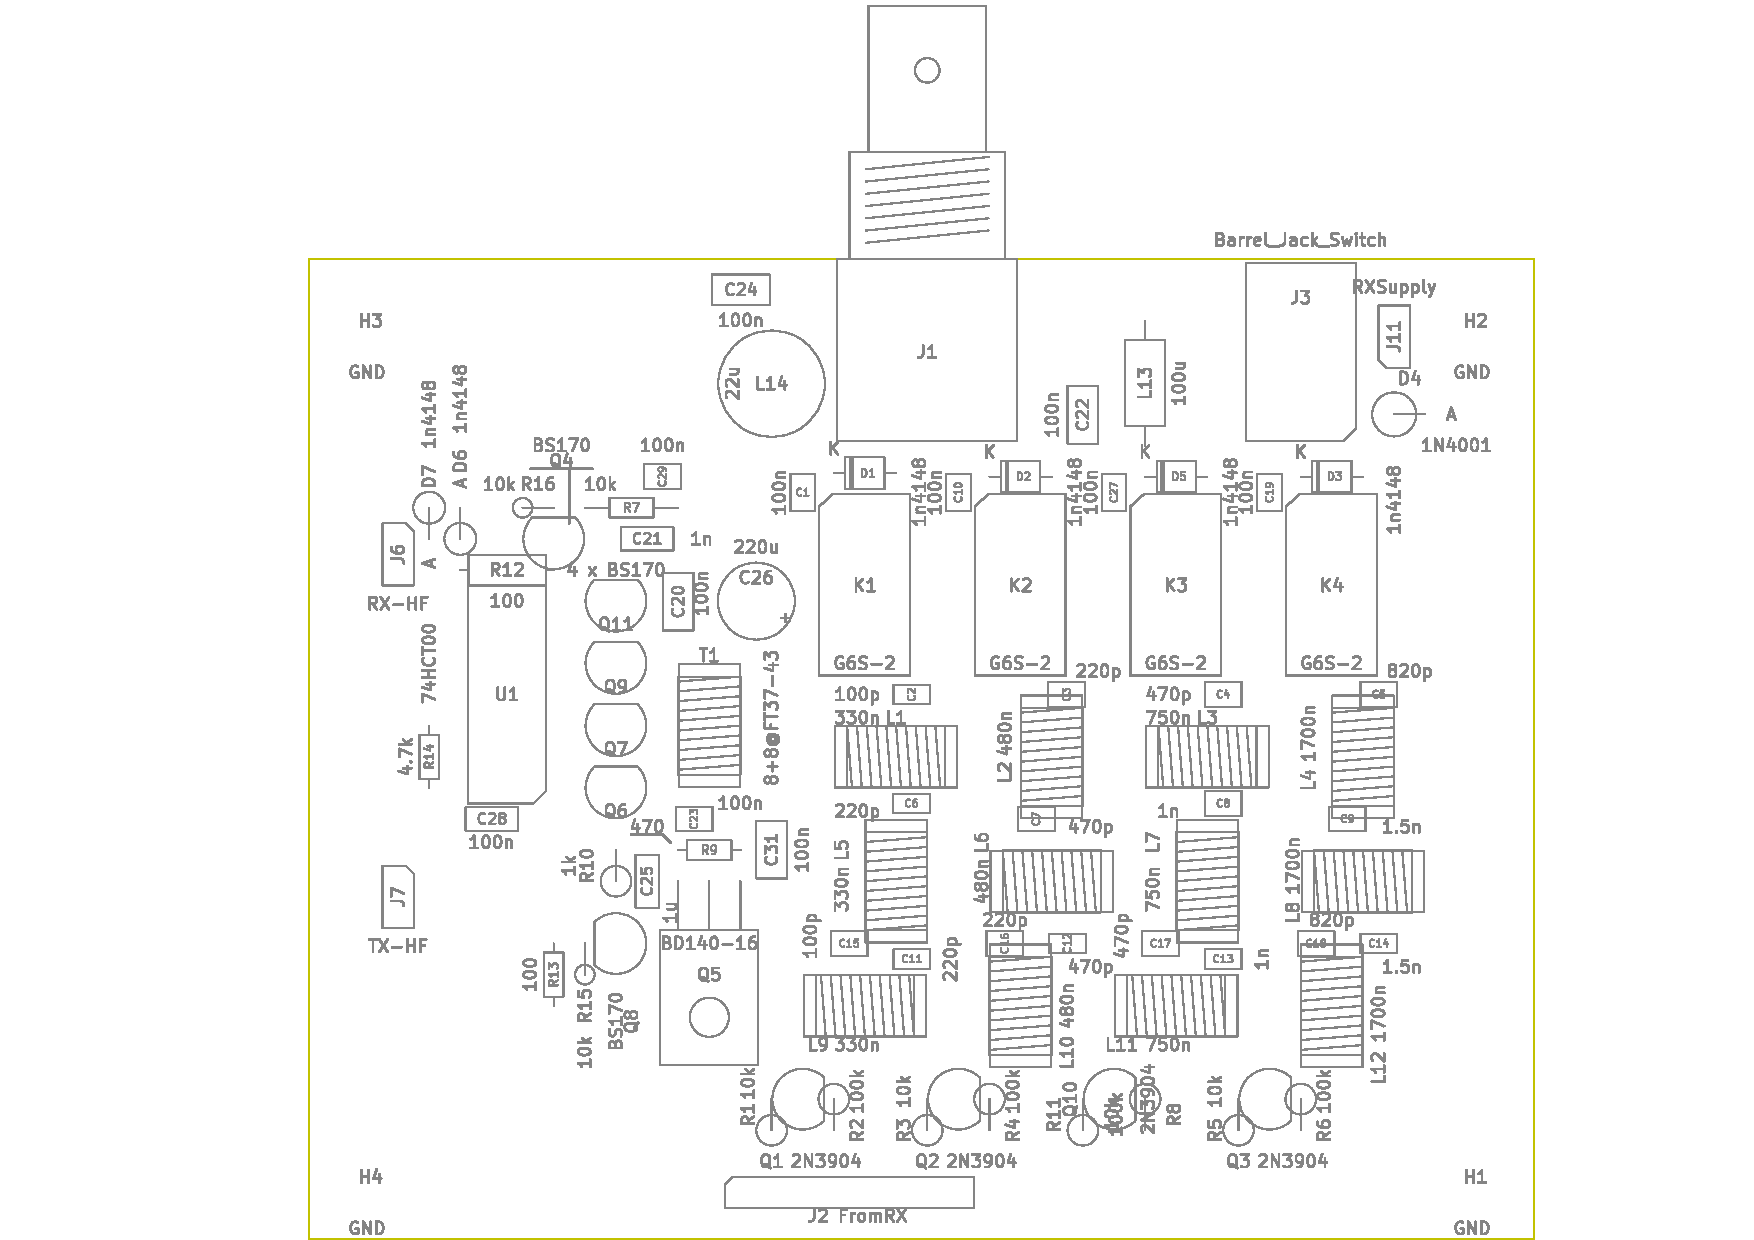
\includepdf[landscape=true, addtotoc={
 1, subsection, 1, Component Placement \& Values, pacomp}]{fig/pa_values.pdf}
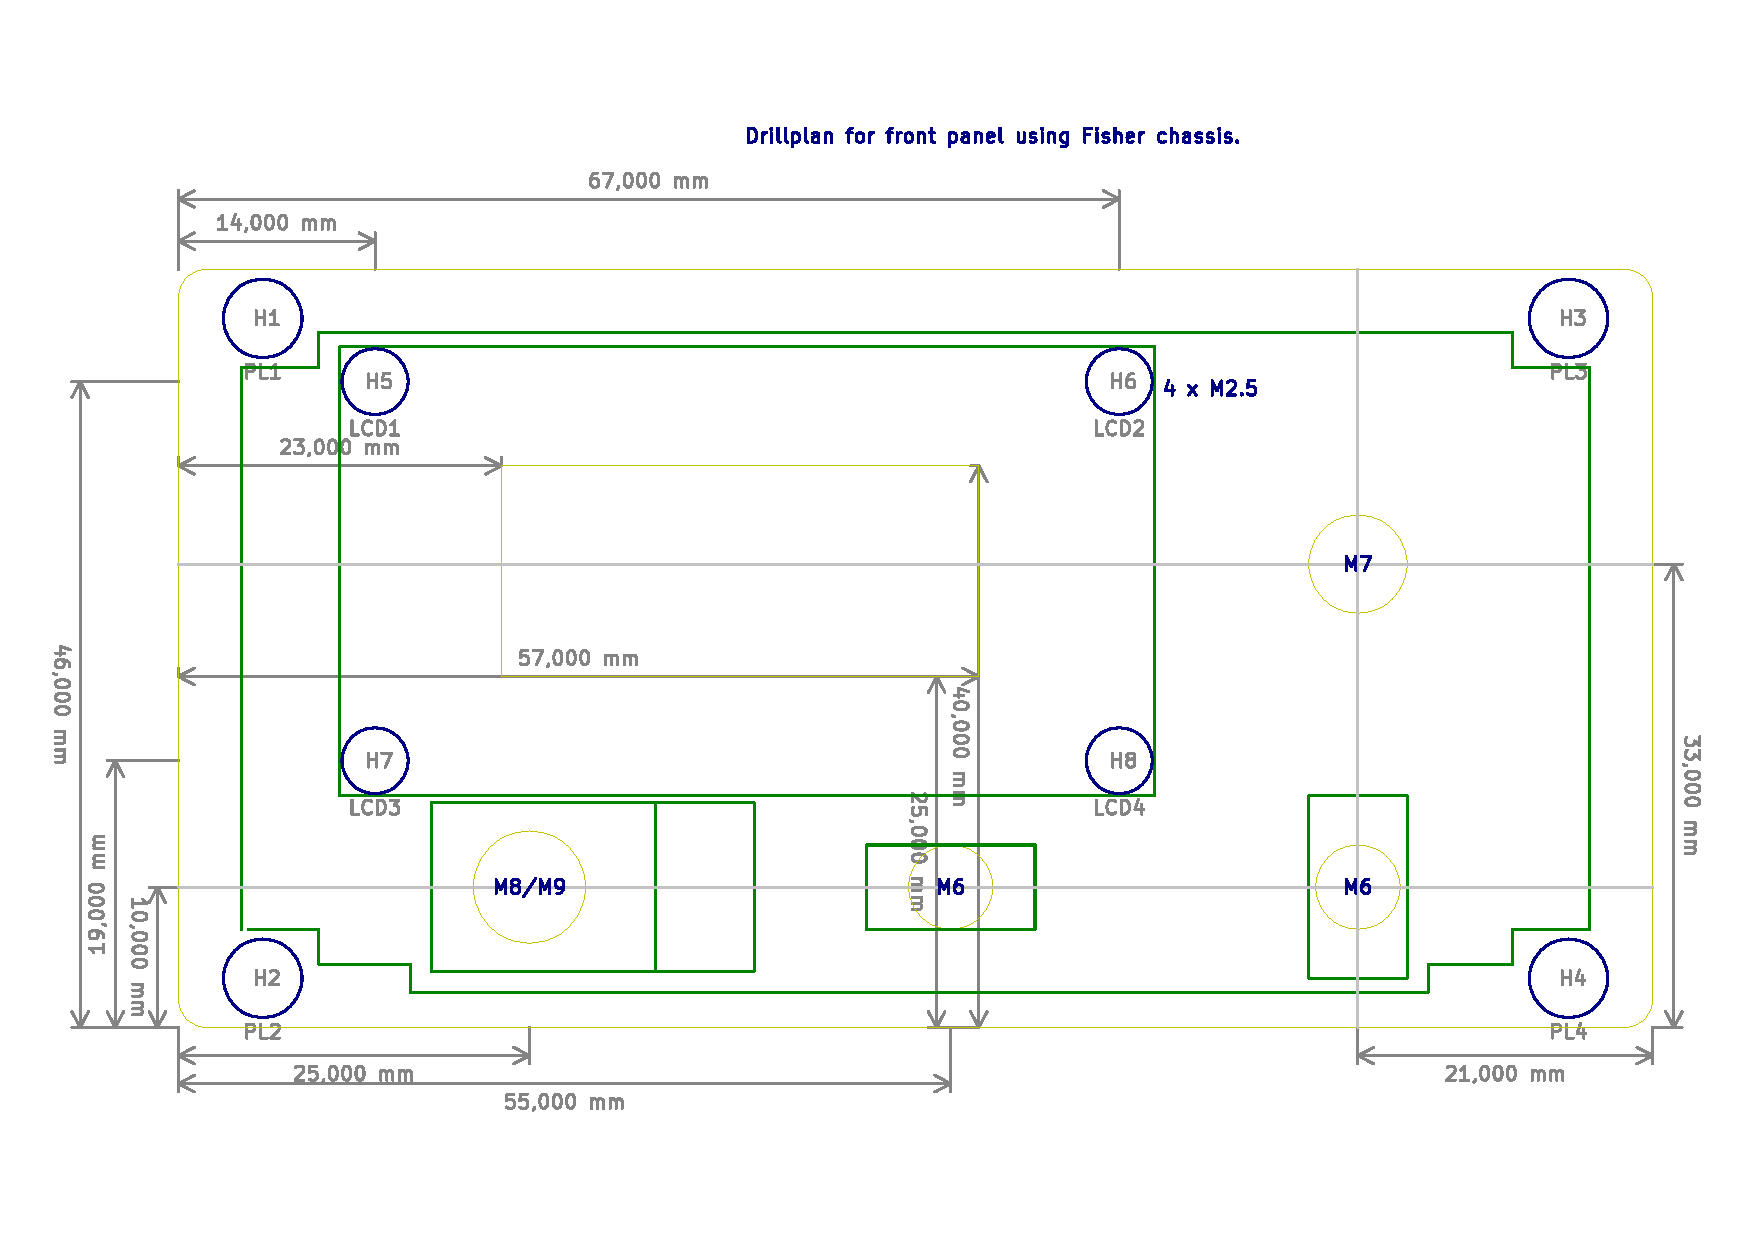
\includepdf[landscape=true, addtotoc={
 1, section, 1, Drill Plan, drillfront}]{fig/drill_front.pdf}
\end{document}